\documentclass{beamer}
\mode<presentation>
{
  \usetheme{Darmstadt}        % or try default, Darmstadt, Warsaw, Darmstadt ,Berkeley,...
  \usecolortheme{orchid} % or try albatross, beaver, crane,whale,orchid,spruce,...
  \usefonttheme{serif}    % or try default, structurebold,serif ...
  \setbeamertemplate{navigation symbols}{}
  \setbeamertemplate{caption}[numbered]
  \setbeamercovered{transparent}
  \setbeamertemplate{footline}
} 
\addtobeamertemplate{block begin}{\pgfsetfillopacity{0.8}}{\pgfsetfillopacity{1}}
\addtobeamertemplate{block alerted begin}{\pgfsetfillopacity{0.8}}{\pgfsetfillopacity{1}}
\addtobeamertemplate{block example begin}{\pgfsetfillopacity{0.8}}{\pgfsetfillopacity{1}}
% \usepackage[total={6.0in,8.0in}]
% \usepackage[brazil]{babel}
\usepackage[brazil]{babel}
\usepackage{lmodern}
\usepackage[utf8x]{inputenc}
% \usepackage[utf8]{inputenc}
\usepackage{cancel}
\usepackage{bigints}
%\usepackage{hyperref}
%\usepackage{chemfig}
%\usepackage[version=3]{mhchem}
\usepackage{pgfpages}
% \usepackage{ebgaramond}
\usepackage{verbatim}
\usepackage{wasysym}
\usepackage{multicol}
\usepackage{booktabs}
\usepackage{longtable}
\usepackage{multirow}
\usepackage{bigstrut}
\usepackage{caption}
\captionsetup{compatibility=false}
\usepackage{subcaption}
\usepackage{enumerate}
\pgfpagesuselayout{resize to}[%
  physical paper width=8in, physical paper height=6in]

  

\newcommand{\linesH}[1]{\rule{\linewidth}{#1}}
%\title{Minicurso \LaTeX}
%\subtitle{Semana Acadêmica da Física - FURG}
%\author{\\
%\textsc{Geferson Lucatelli}\footnote{\texttt{gefersonlucatelli@furg.br}}\\
%\textsc{Gabriel Lauffer Ramos}\footnote{\texttt{gabriel...}}\\
%\textsc{Vinícius Marcelo Becker}\footnote{\texttt{viniciusbecker@furg.br}}}

\title{Minicurso \LaTeX}
\subtitle{Semana Acadêmica da Física - FURG}
\date[2016]{Rio Grande, RS}
\author{\textsc{Gabriel Lauffer Ramos} \inst{1}\footnote[1]{\texttt{gabriellramos@gmail.com}},
\textsc{Geferson Lucatelli}\inst{1} \footnote[2]{\texttt{gefersonlucatelli@furg.br}},
\textsc{Vinícius Marcelo Becker}\inst{1} \footnote[3]{\texttt{viniciusbecker@furg.br}}
}
\institute[IMEF]{{\large{Universidade Federal do Rio Grande}}\\
\inst{1}Instituto de Matemática, Estatística e Física}
\logo{
\includegraphics[scale=.04]{furg.png} / 

\includegraphics[scale=.03]{imef.jpg}}

\begin{document}
% \fontsize{8pt}{15.0}\selectfont
\begin{frame}
  \maketitle
\end{frame}

{\fontsize{10pt}{10.0}\selectfont

\begin{frame}{Sumário}
\begin{multicols}{2}
  \tableofcontents
\end{multicols}
\end{frame}

}
\section{Módulo I}
\begin{frame}
\begin{center}
 {\Huge  Módulo I}
\end{center}
\end{frame}


\subsection{Instalação do \LaTeX}

\begin{frame}[fragile]{Instalação \LaTeX\  Linux}
% \begin{frame}[fragile=singleslide]\frametitle{Instalação \LaTeX\  Linux}
No sistema operacional Ubuntu e seus derivados, a instalação do \LaTeX\ e seus pacotes é simples e fácil. Basta introduzir os seguintes comandos no terminal:  
\begin{itemize}
 \item \verb|$ sudo apt-get install texlive-full| \quad $\sim$ \quad 3.7 Gb
 \item \verb|$ sudo apt-get install texmaker|
 \item \verb|$ sudo apt-get install abntex|
\end{itemize}
Após a instalação dos pacotes abra o Texmaker com \verb|$ texmaker|.
\end{frame}

\begin{frame}{Instalação \LaTeX\ Windows}
Para a instalação do \LaTeX no Windows, basta fazer o download e instalação de:
\begin{itemize}
 \item MiKTeX e Texmaker:  \url{http://cluster.ft.unicamp.br/wiki/doku.php?id=ambiente:latex_windows};
 \item baixe a versão correta para seu computador;
\item outra alternativa além do MiKTeX, é baixar o \TeX\ Live: \url{https://www.tug.org/texlive/acquire-netinstall.html} em \emph{install-tl-windows.exe} \quad $\sim$ \quad 4.4 Gb
 \end{itemize}
\end{frame}

\subsection{Estrutura de um documento}

\begin{frame}
 \frametitle{Estrutura de um documento}
 Um documento em \LaTeX  é composto basicamente de duas partes:
 \begin{itemize}
 \item preâmbulo: aqui são feitas as declarações sobre a classe do documento, configurações globais e o carregamento dos pacotes;
 \item corpo: contém o texto propriamente dito;
 \end{itemize}
\end{frame}

\subsubsection{Preâmbulo}

\begin{frame}[fragile]
 \frametitle{Preâmbulo -- Classe do Documento}
 \begin{itemize}
  \item Classe do documento: Todo arquivo em \LaTeX\ deve iniciar com a declaração 
de classe do documento, feito através do comando:\\
  \begin{center}
  \verb| \documentclass[opções]{classe} |
  \end{center}
  \item As opções se referem às seguintes configurações:
    \begin{itemize}
     \item Tamanho da fonte do texto (10pt, 12pt, 14pt)
     \item Formato do papel (a4paper)
     \item Número de colunas (onecolumn, twocolumn)
     \item Orientação da folha (landscape, portrait)
     \item Impressão só frente ou frente e verso (oneside, twoside)
    \end{itemize}
 \end{itemize}
\end{frame}

\begin{frame}[fragile]
 \frametitle{Preâmbulo -- Classe do Documento}
 \begin{itemize}
  \item Classe do documento: Todo arquivo em \LaTeX\ deve iniciar com a declaração 
de classe do documento, feito através do comando:\\
  \begin{center}
  \verb| \documentclass[opções]{pacote} |
  \end{center}
  \item Aguns tipos de classe são:
    \begin{itemize}
     \item article
     \item beamer
     \item book
     \item letter
     \item report
    \end{itemize}
 \end{itemize}
\end{frame}

\begin{frame}[fragile]
 \frametitle{Preâmbulo -- Pacotes}
 \begin{itemize}
  \item  A declaração dos pacotes é feita através do comando:\\
  \begin{center}
  \verb| \usepackage[opções]{classe} |
  \end{center}
  \item Alguns pacotes importantes:
    \begin{itemize}
     \item \textbf{babel}: Pacote para hifenização automática do texto. Para usar português do Brasil, usamos \textit{brazil} como opção;
     \item \textbf{inputenc}: Especifica o tipo de encoding utilizado na fonte do documento. As opcões mais usadas são o \textit{utf8} e o \textit{latin1}. Com este pacote, caracteres com acentos podem ser digitados diretamente no código fonte, sem a necessidade de utilizar comandos especiais;
     \item \textbf{amssymb, amsmath}: Habilitam alguns caracteres e comandos matemáticos especiais.
     \item \textbf{geometry}: Pacote para configurar as dimensões das margens e largura
da folha;
    \end{itemize}
 \end{itemize}
\end{frame}

\subsubsection{Corpo}

\begin{frame}[fragile]
 \frametitle{Corpo}
  \begin{itemize}
   \item O corpo do documento consiste em tudo aquilo que está inserido entre os
seguintes comandos:\\
    \begin{center}
     \verb| \begin{document} |\\
      .\\
      .\\
      .\\
     \verb| \end{document} |
    \end{center}
   \item Todos os capítulos, seções e subseções devem estar inseridos entre estes
comandos; 
   \item O que for escrito após o fim do documento será ignorado pelo compilador 
  \end{itemize} 
\end{frame}

\subsection{Organização dos Documentos}

\begin{frame}
 \frametitle{Organização dos Documentos}
  \begin{itemize}
   \item A organização dos arquivos é muito importante. Recomendamos que:
    \begin{itemize}
     \item para cada documento, se crie uma nova pasta, na qual ficarão todos os arquivos relacionados ao documento;
     \item dentro desta pasta, é interessante criar uma nova pasta, na qual serão colocadas todas as imagens que aparacerão no documento;
    \end{itemize} 
  \end{itemize} 
\end{frame}

\section{Módulo II - Elementos do Texto}

\begin{frame}
\begin{center}
 {\Huge  Módulo II}
 \\
 {\normalsize Elementos do Texto}
\end{center}
\end{frame}

\subsection{Comandos de Texto}

\begin{frame}[fragile]
\frametitle{Comandos de Texto}
\begin{itemize}
\item Palavras: Separadas por espaços em branco.
\item Parágrafos: Separados por linhas em branco ou \verb| \\ |
\begin{itemize}
\item Diferente dos processadores de texto comuns, um novo parágrafo não é definido pela tecla ''Enter" e sim por uma linha em branco ou pelo comando \verb| \\ |
\end{itemize}
\item Caracteres especiais: Alguns símbolos precisam ser precedido de uma barra \verb|\| para serem compilados. 
\begin{itemize}
\item Os comandos \verb|\&|, \verb|\$|, \verb|\%|, \verb|\_| geram os símbolos \&, \$, \%, \_
\end{itemize}
\item Comentários: Qualquer caractere precedido pelo símbolo \% será interpretado como um comentário e não será compilado no documento final
\end{itemize}
\end{frame}

\subsection{Seções}

\begin{frame}[fragile]{Seções - Títulos e Subtítulos}

No \LaTeX \ títulos e subtítulos são chamados de \texttt{section} e \texttt{subsection}. Os comandos possuem a forma,

\center{\verb|\section{título}|}

\flushleft{
em que \texttt{título} é o título desejado.}

O \LaTeX  \ numera automaticamente os títulos e subtítulos. Se a numeração não é desejada podemos utilizar um \verb|*| no comando antes das chaves.

\center{\verb||}

\end{frame}

\begin{frame}[fragile]{Seções - Títulos e Subtítulos}
\center{Exemplo de títulos:}
\vspace{0.2cm}
\begin{columns}
\begin{column}{0.4\textwidth}
%\centering
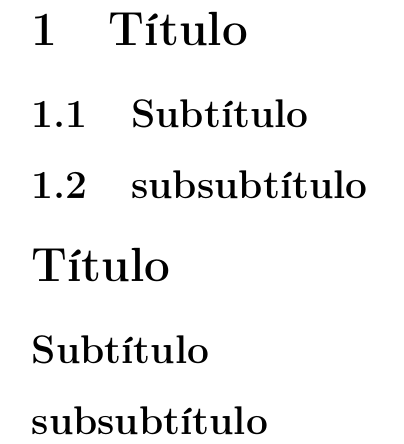
\includegraphics[scale=0.3]{exemplo_titulo.png}
\end{column}
%
\begin{column}{0.6\textwidth}
\verb|\section{Título}| \\
\verb|\subsection{Subtítulo}| \\
\verb|\subsubsection{subsubtítulo}| \\
\verb|\section*{Título}| \\
\verb|\subsection*{Subtítulo}| \\
\verb|\subsubsection*{subsubtítulo}| \\
\end{column}

\end{columns}
\end{frame}

\begin{frame}{Exercício - Títulos}
Para as próximas etapas:
\begin{columns}
\begin{column}{0.5\textwidth}
\begin{itemize}
\item Criar um título e dois subtítulos no documento.
\begin{itemize}
\item Título: Modificadores
\item Subtitulo 1: Texto
\item Subtitulo 2: Tamanho
\end{itemize}
\end{itemize}
\end{column}


\begin{column}{0.5\textwidth}
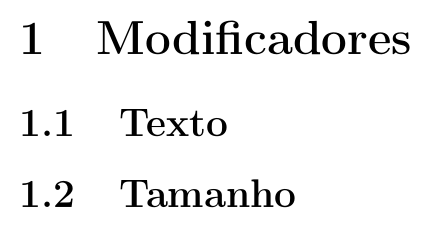
\includegraphics[scale=0.3]{exerc_titulos.png}
\end{column}

\end{columns}

\end{frame}

\begin{frame}[fragile]{Exercício - Títulos (Solução)}
\begin{verbatim}
\begin{document}
\section{Modificadores}
\subsection{Texto}
\subsection{Tamanho}
\end{document}
\end{verbatim}
\end{frame}

\subsection{Modificadores}

\begin{frame}[fragile]{Modificadores}
\begin{itemize}
\item Negrito: \verb|\textbf{Texto}| produz \textbf{Texto}
\item Itálico: \verb|\textit{Texto}| produz \textit{Texto}
\item Sublinhado: \verb|\underline{Texto}| produz \underline{Texto}
\item Letra de código: \verb|\texttt{Texto}| produz \texttt{Texto}
%\item Caixa alta: \verb|\textsc{Texto}| produz \texts
\end{itemize} 
\end{frame}

\begin{frame}[fragile]{Modificadores de tamanho I}
\begin{itemize}
\item os modificadores de tamanho devem ser colocados entre chaves \{ \verb|\modificador| Texto \}
\end{itemize}
\{ \verb|\tiny| Texto \} produz: {\tiny Texto} 

\{ \verb|\scriptsize| Texto \} produz: {\scriptsize Texto}

\{ \verb|\footnotesize| Texto \} produz: {\footnotesize Texto}

\{ \verb|\small| Texto \} produz: {\small Texto}

\{ \verb|\normalsize| Texto \} produz:  {\normalsize Texto}


\end{frame}

\begin{frame}[fragile]{Modificadores de tamanho II}
\{ \verb|\large| Texto \} produz: {\large Texto}

\{ \verb|\Large| Texto \} produz: {\Large Texto}

\{ \verb|\LARGE| Texto \} produz: {\large Texto}

\{ \verb|\huge| Texto \} produz: {\huge Texto}

\{ \verb|\Huge| Texto \} produz: {\Huge Texto}
\end{frame}


\begin{frame}{Exercício - Modificadores}

\begin{itemize}
\item Escrever dentro do subtítulo \textbf{Texto} alguma frase utilizando texto em \textbf{Negrito} ou \textit{Itálico} (ou algum outro modificador).
\item Escrever dentro do subtítulo \textbf{Tamanho} alguma frase modificando o tamanho do texto.
\item Obs: Se quiserem, tentem utilizar caracteres especiais!
\end{itemize}
\end{frame}

\begin{frame}{Exercício - Modificadores - Exemplo}

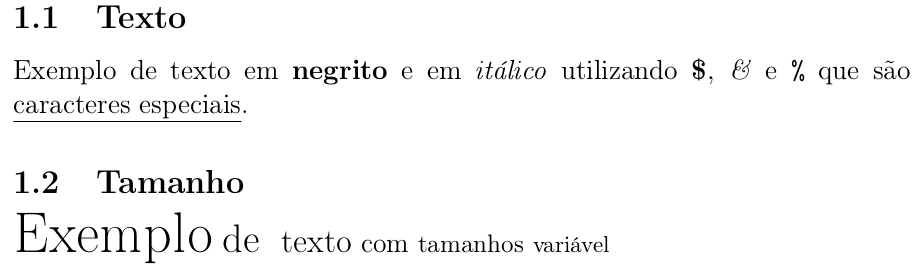
\includegraphics[scale=0.32]{exerc_modificadores.png}

\end{frame}

\begin{frame}[fragile]{Exercício - Modificadores (Solução)}
\begin{verbatim}
\subsection{Texto}

Exemplo de texto em \textbf{negrito} e em \textit{itálico} 
utilizando \textbf{\$}, \textit{\&} e \texttt{\%} 
que são \underline{caracteres especiais}.

\subsection{Tamanho}

{\Huge Exemplo} {\Large de } {\large texto} 
{\normalsize com} {\small tamanhos}
 {\footnotesize variável}  
\end{verbatim}
\end{frame}

\subsection{Espaçamento}

\begin{frame}[fragile]{Espaçamento I}
O \LaTeX \ manipula os espaçamentos automaticamente, porém nem sempre o documento compilado fica do formato desejado. Portanto, existem alguns comandos para manipular os espaçamentos.

\begin{itemize}
\item \verb|\hspace{tamanho}| produz espaçamento horizontal
\item \verb|\vspace{tamanho}| produz espaçamento vertical
\item \verb|\\[tamanho]]| produz espaçamento vertical antes de começar uma nova linha
\end{itemize}
Estes três comandos acima necessitam da opção \texttt{tamanho} que é definido pelo usuário. Esta opção deve ser um numero seguido de sua unidade. Por exemplo,
\begin{itemize}
\item \verb| \hspace{5cm}|
\item \verb| \\[8mm]|
\end{itemize}
\end{frame}

\begin{frame}[fragile]{Espaçamento II}
Existem outros comandos que não necessitam de um tamanho especificado pelo usuário:
\begin{itemize}
\item \verb|\hfill| adiciona espaços horizontais para preencher a largura da pagina
\item \verb|\vfill| adiciona espaços verticais para preencher a altura da pagina
\item \verb|\newline| inicia uma nova linha
\item \verb|\newpage| inicia uma nova página
\item \verb|\noindent| remove o espaçamento antes do parágrafo.
\end{itemize}
\end{frame}

\begin{frame}[fragile]{Espaçamento III}
No \LaTeX \ também é possível modificar o espaçamento entre linhas. Há mais de uma forma de modificar este espaçamento. Para isto, teremos que adicionar ao preambulo o pacote,
\center{ \verb| \usepackage{setspace} | }

O espaçamento pode ser modificado utilizando os comandos:
\begin{itemize}
\item \verb|\singlespacing| espaçamento simples entre linhas 
\item \verb|\onehalfspacing| espaçamento $1,5$
\item \verb|\doublespacing| espaçamento duplo
\end{itemize}
\end{frame}

\begin{frame}{Espaçamento III}
Um desses comandos pode ser adicionado no preambulo para definir o espaçamento para todo o documento. Porém, é possível modificar o espaçamento entre linhas local adicionando o comando na região do texto em que se quer modificar o espaçamento mas deve-se terminar esta região com outro comando para retornar ao espaçamento desejado
\end{frame}


\begin{frame}{Exercício - Espaçamento}

\begin{itemize}
\item Definir espaçamento duplo no documento (adicionar o pacote e o comando no preambulo)
\item Compilar
\item Adicionar um espaçamento vertical entre os subtítulos \textbf{Texto} e \textbf{Tamanho}
\item Compilar
\end{itemize}

\end{frame}
\subsection{Ambientes}

\begin{frame}[fragile]{Ambientes}
Um ambiente e uma região do texto que tem um tratamento especial.  Um ambiente é iniciado com \verb|\begin{}| e terminado com \verb|\end{}| com o nome do ambiente entre as chaves. Exemplos de ambientes são:
\begin{itemize}
\item Listas
\begin{itemize}
\item \verb|itemize|
\item \verb|enumerate|
\end{itemize}
\item Alinhamento
\begin{itemize}
\item \verb|\flushleft|
\item \verb|\flushright|
\item \verb|\center|
\end{itemize}
\item Matemático
\begin{itemize}
\item \verb|equation|
\item \verb|eqnarray|
\item \verb|align|
\end{itemize}
\item Tabelas
\item Figuras
\end{itemize}
\end{frame}

\subsubsection{Listas por itens}

\begin{frame}[fragile]{Listas}
Os ambientes de listas possuem o mesmo modelo de código.
\center{
\verb|\begin{ambiente}| \\
\verb|\item| Texto \\ 
\verb|\item| Texto \\ 
\verb|\end{ambiente}| \\
}
\end{frame}

\begin{frame}[fragile]{Listas por itens - \texttt{itemize}}
\center{Exemplo de lista:}
\vspace{0.2cm}
\begin{columns}
\begin{column}[t]{0.5\textwidth}
\begin{itemize}
\item Primeiro item
\item Segundo item
\item Terceiro item
\end{itemize}
\end{column}

\begin{column}[t]{0.5\textwidth}
\verb|\begin{itemize}| \\
\verb|\item Primeiro item| \\
\verb|\item Segundo item| \\
\verb|\item Terceiro item| \\
\verb|\end{itemize}|
\end{column}

\end{columns}

\end{frame}

\begin{frame}[fragile]{ Sublistas - \texttt{itemize}}
\center{Exemplo de sublista:}
\vspace{0.2cm}

\begin{columns}
\begin{column}[t]{0.5\textwidth}
\begin{itemize}
\item Primeiro item
\begin{itemize}
\item Primeiro subitem
\item Segundo subitem
\end{itemize}
\item Segundo item
\end{itemize}
\end{column}

\begin{column}[t]{0.5\textwidth}
%\begin{verbatim}
%\begin{itemize}
%\item Primeiro item
%	\begin{itemize}
%	\item Primeiro subitem
%	\item Segundo subitem
%	\end{itemize}
%\item Segundo item
%\end{itemize}
%\end{verbatim}
\verb|\begin{itemize}| \\
\verb|\item Primeiro item| \\
\hspace{.5cm}\verb|\begin{itemize}| \\
\hspace{.5cm}\verb|\item Primeiro subitem| \\
\hspace{.5cm}\verb|\item Segundo subitem| \\
\hspace{.5cm}\verb|\end{itemize}| \\
\verb|\item Segundo item| \\
\verb|\end{itemize}|
\end{column}

\end{columns}

\end{frame}

\subsubsection{Lista ordenadas}
\begin{frame}[fragile]{Listas ordenadas}
O ambiente \texttt{enumerate} gera listas numeradas.

\begin{columns}
\begin{column}[t]{0.5\textwidth}
\begin{figure}
\centering
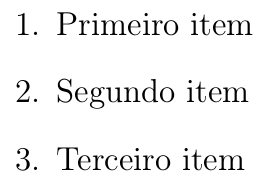
\includegraphics[width=0.6\textwidth]{enumerate_simples.png}
\end{figure}
\end{column}
%
\begin{column}[t]{0.5\textwidth}
\begin{verbatim}
\begin{enumerate}
\item Primeiro item
\item Segundo item
\item Terceiro item
\end{enumerate}
\end{verbatim}
\end{column}

\end{columns}

\end{frame}

\begin{frame}[fragile]{Sublistas ordenadas}
e também sublistas.

\begin{columns}
\begin{column}[t]{0.5\textwidth}
\begin{figure}
\centering
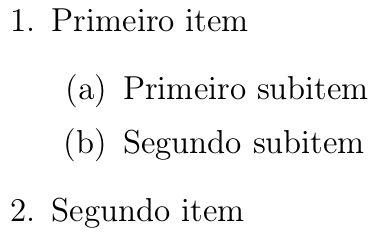
\includegraphics[width=0.8\textwidth]{enumerate_sublista.png}
\end{figure}
\end{column}

\begin{column}[t]{0.5\textwidth}

\verb|\begin{enumerate}| \\
\verb|\item Primeiro item| \\
\hspace{.5cm}\verb|\begin{enumerate}| \\
\hspace{.5cm}\verb|\item Primeiro subitem| \\
\hspace{.5cm}\verb|\item Segundo subitem| \\
\hspace{.5cm}\verb|\end{enumerate}| \\
\verb|\item Segundo item| \\
\verb|\end{enumerate}|
\end{column}
\end{columns}

\end{frame}

\begin{frame}[fragile]{\texttt{enumerate}}
O ambiente \texttt{enumerate} nos permite controlar o formato da lista. Para isto, precisamos adicionar no preambulo o pacote,
\center{\verb|\usepackage{enumerate}|}

a modificação é feita ao iniciar o ambiente, da seguinte forma,
\center{\verb|\begin{enumerate}[opção]|}

as opções podem ser:

\begin{enumerate}[i)]
\item \verb|i)|
\end{enumerate}
\begin{enumerate}[(i)]
\item \verb|(i)|
\end{enumerate}
\begin{enumerate}[I)]
\item \verb|I)|
\end{enumerate}
\begin{enumerate}[(a)]
\item \verb|(a)|
\end{enumerate}
\end{frame}

\begin{frame}[fragile]{Listas - Exercícios}
Reproduzir a lista abaixo!
\begin{figure}
\centering
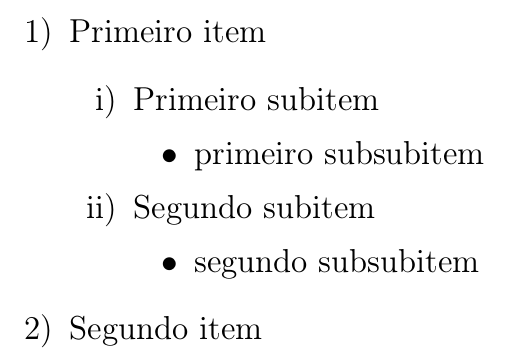
\includegraphics[scale=0.3]{exercicio_lista.png}
\end{figure}
\end{frame}

\begin{frame}[fragile]{Listas - Exercícios (solução)}
\verb|\begin{enumerate}[1)]| \\
\verb|\item Primeiro item| \\
\hspace{.5cm}\verb|\begin{enumerate}[i)]| \\
\hspace{.5cm}\verb|\item Primeiro subitem| \\
\hspace{1cm}\verb|\begin{itemize}| \\
\hspace{1cm}\verb|\item primeiro subsubitem| \\
\hspace{1cm}\verb|\end{itemize}| \\
\hspace{.5cm}\verb|\item Segundo subitem| \\
\hspace{1cm}\verb|\begin{itemize}| \\
\hspace{1cm}\verb|\item segundo subsubitem| \\
\hspace{1cm}\verb|\end{itemize}| \\
\hspace{.5cm}\verb|\end{enumerate}| \\
\verb|\item Segundo item| \\
\verb|\end{enumerate}|
\end{frame}

\subsubsection{Alinhamento}

\begin{frame}[fragile]{Alinhamento}

Normalmente \LaTeX \ mantêm os textos com o alinhamento "Justificado". Para modificar o alinhamento, podemos utilizar 3 opções:
\begin{itemize} 
\item \texttt{flushleft} ,Alinhado à esquerda
\item \texttt{flushright}, Alinhado à direita
\item \texttt{center}, Centralizado
\end{itemize}
O código para utilizar estes alinhamento é o seguinte,

\begin{verbatim}
\begin{alinhamento}
texto, frase ou parágrafo
\end{alinhamento}
\end{verbatim}
\end{frame}

\subsubsection{Fórmulas Matemáticas}

\begin{frame}
 \frametitle{Fórmulas Matemáticas}
  \begin{itemize}
   \item 
   \item Espaços em branco são ignorados pelo compilador e, como padrão, todas as letras são escritas em itálico; 
  \end{itemize}
\end{frame}

\begin{frame}[fragile]
 \frametitle{Fórmulas Matemáticas}
  \begin{itemize}
   \item As equações matemáticas podem ser escritas de maneiras diferentes:
    \begin{itemize}
     \item O comando \verb|$x+1=1$| produz $x+1=1$;
     \item O comando \verb|$$x+1=1$$| produz $$x+1=1;$$
     \item O comando \\
                     \verb|\begin{equation}|\\
                     \verb|x+1=1|\\
                     \verb|\end{equation}|\\  
     produz \begin{equation}
              x+1=1;
             \end{equation} 
    \end{itemize}
  \end{itemize}
\end{frame}

\begin{frame}[fragile]
 \frametitle{Fórmulas Matemáticas}
  \begin{itemize}
   \item As equações matemáticas podem ser escritas de maneiras diferentes:
    \begin{itemize}
     \item O comando \\
                     \verb|\begin{eqnarray}|\\
                     \verb|x+1&=&1\nonumber\\|\\
                     \verb|x&=&0|\\
                     \verb|\end{eqnarray}|\\  
     produz \begin{eqnarray}
              x+1&=&1\nonumber\\
              x&=&0
             \end{eqnarray} 
    \end{itemize}
  \end{itemize}
\end{frame}

\begin{frame}[fragile]
 \frametitle{Fórmulas Matemáticas}
  \begin{itemize}
   \item A seguir, apresentamos uma lista de caracteres do alfabeto grego e o respectivo comando:
    \begin{figure}[h]
    \centering
    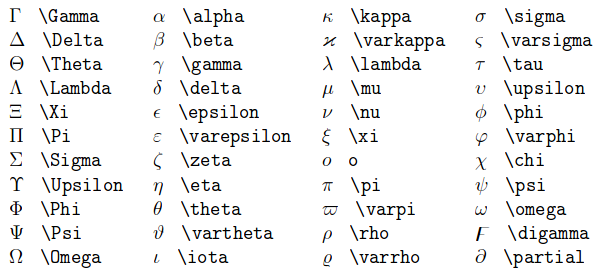
\includegraphics[scale=0.46]{letras_gregas}
    \end{figure}
  \end{itemize}
\end{frame}

\begin{frame}
 \frametitle{Fórmulas Matemáticas}
Fontes: é possível modificar o estilo de fonte utilizada dentro do ambiente matemático. Alguns exemplos são:
\begin{figure}
	\centering
	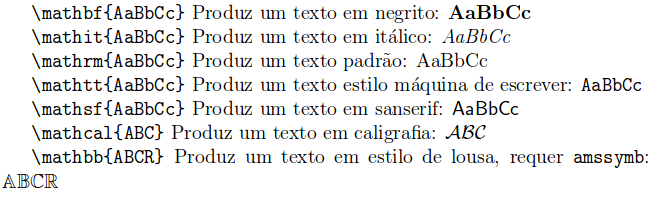
\includegraphics[width=0.7\linewidth]{fontes.png}
	\caption{}
	\label{fig:fontes}
\end{figure}

\end{frame}	

\subsection{Inserindo Tabelas}

\begin{frame}[fragile]
 \frametitle{Inserindo Tabelas}
  \begin{itemize}
   \item Uma tabela é especificada pelo ambiente \verb| tabular |;
   \item A criação de uma tabela é feita da seguinte forma:
   \verb| \begin{tabular}{espec} |\\
em que o argumento \verb| espec | especifica a quantidade de colunas e o seu alinhamento:    
    \begin{itemize}
     \item $|$ adiciona uma linha vertical;
     \item \textbf{l} indica uma coluna alinhada à esquerda;
     \item \textbf{r} indica uma coluna alinhada à direita;
     \item \textbf{c} indica uma coluna com texto centralizado;
    \end{itemize} 
   \item Quanto ao preenchimento da tabela, utilizamos:
    \begin{itemize}
     \item \verb|\&| para passar para a próxima coluna;
     \item \verb| \\ | para terminar uma linha e criar para uma nova;
     \item \verb|\hline| para criar uma linha horizontal.
    \end{itemize} 
  \end{itemize}
\end{frame}
    
\begin{frame}[fragile]
 \frametitle{Inserindo Tabelas}
  \begin{itemize}
   \item Uma tabela pode ser inserida dentro do ambiente \verb|table|, o que faz dela
um objeto flutuante;
   \item Vantagens de utilizar esse tipo de ambiente:
    \begin{itemize}
     \item posição correta da tabela no texto;
     \item permite a inserção de rótulos e legendas;
     \item faz com que a tabela apareça em um índice de tabelas;
    \end{itemize}
   \item Para usar este ambiente é preciso usar o comando\\ 
    \verb|\begin{table}[pos]|\\
em que \verb|pos| indica a posição desejada para se posicionar a tabela verticalmente na página: 
   \begin{itemize}
    \item \textbf{h} no local onde o texto ocorreu;
    \item \textbf{t} no topo da página;
    \item \textbf{b} no fim da página;
    \item \textbf{p} em uma página especial contendo somente objetos flutuantes;
   \end{itemize}
  \end{itemize}
\end{frame}

\begin{frame}[fragile]
 \frametitle{Inserindo Tabelas}
  \begin{itemize}
   \item Para adicionar uma legenda usamos, ainda dentro do ambiente \verb|table|, o comando\\
   \verb|\caption{legenda}|
   \item A seguir apresentamos uma tabela criada como objeto flutuante e os comandos utilizados para que fosse gerada:
  \end{itemize}
\end{frame}

\begin{frame}[fragile]
 \frametitle{Inserindo Tabelas}
\begin{table}[h]
\begin{tabular}{c|c} 
   \toprule
    \textbf{RS}             &\textbf{Temperatura Máxima} ($^{\circ}C)$\\
   \midrule
   Porto Alegre             &39\\ \hline
   Santa Maria              &40\\ \hline
   Rio Grande               &40\\ \hline
   Pelotas                  &40\\ \hline
   Caxias do Sul            &38\\ \hline 
   \bottomrule
\end{tabular}
\end{table}
\end{frame}

\begin{frame}[fragile]
 \frametitle{Inserindo Figuras}
 \centering
 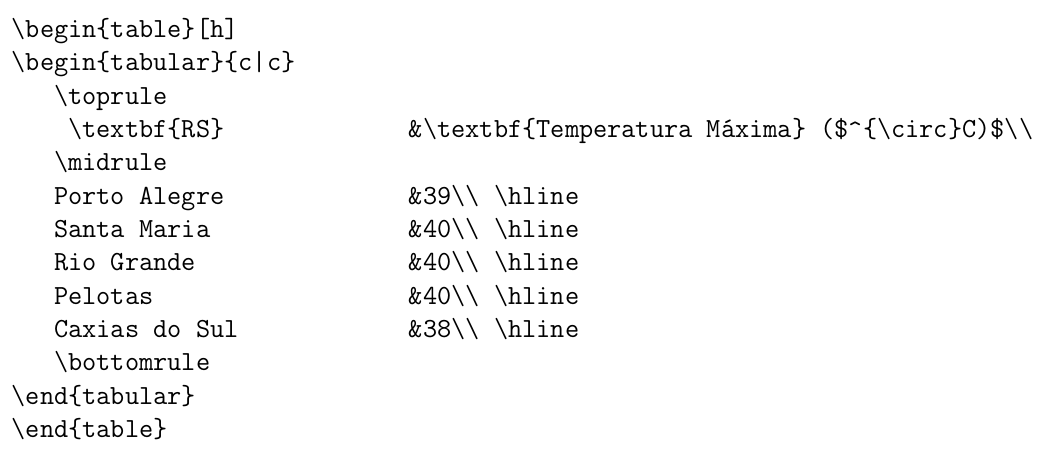
\includegraphics[scale=0.3]{exemplo_tabela}
\end{frame}

\begin{frame}
 \frametitle{Exemplos de Tabelas}
  \begin{center}
   \resizebox{8cm}{!}{\begin{tabular}{cccc} 
   \toprule
   \textbf{Qualidade da construção}       &\textbf{a}                       &\textbf{b}                     &\textbf{c}\\
   \midrule
   Boa vedação                   &0,15                    &0,010                 &0,007\\
   Média                         &0,20                    &0,015                 &0,014\\
   Má vedação                    &0,25                    &0,020                 &0,022\\
   \bottomrule 
                       \end{tabular}}
  \end{center}

\begin{center}
\begin{tabular}{c|c|c} 
   \toprule
    \textbf{Resistência}              &\textbf{Expressão}                                                       &\textbf{Efeito}                \\
   \midrule
   \multirow{2}{*}{$R_{1}$}           &\multirow{2}{*}{$\displaystyle\frac{1}{h_{i}2\pi r_{1}L}$}               &\multirow{2}{*}{Inalterada}    \\ 
                                      &                                                                         &                               \\ \hline 
   \multirow{2}{*}{$R_{2}$}           &\multirow{2}{*}{$\displaystyle\frac{\ln(r_{2}/r_{1})}{K_{t}2\pi L}$}     &\multirow{2}{*}{Inalterada}    \\ 
                                      &                                                                         &                               \\ \hline
   \multirow{2}{*}{$R_{3}$}           &\multirow{2}{*}{$\displaystyle\frac{\ln(r_{3}/r_{2})}{K_{iso}2\pi L}$}   &\multirow{2}{*}{Aumenta}       \\ 
                                      &                                                                         &                               \\ \hline
   \multirow{2}{*}{$R_{4}$}           &\multirow{2}{*}{$\displaystyle\frac{1}{h_{e}2\pi r_{3}L}$}               &\multirow{2}{*}{Diminui}       \\ 
                                      &                                                                         &                               \\ \hline
   \bottomrule
\end{tabular}
\end{center}
\end{frame}

\begin{frame}
 \frametitle{Exemplo de Tabelas}
  \begin{table}[c]
   \begin{center}
   \resizebox{10cm}{!}{\begin{tabular}{c|c|c|c|c|c} 
   \toprule
    \multirow{2}{*}{\textbf{Material Isolante}}             &\multirow{2}{*}{$Kgf/m^{3}$}        &\multirow{2}{*}{$k\frac{Kcal}{mh^{\circ}C}$}     &\textbf{Resistência}                         &\textbf{Resistência à}                           &\textbf{Permeabilidade}      \\
                                                            &                                    &                                                 &\textbf{Mecânica:}$Kgf/m^{2}$                &\textbf{temperatura:}$^{\circ}C$                 &$g/m.h.mmHg$            \\
   \midrule
   Aço ordinário                                            &7800                                &45 a 50                                          &                                    &                                        &Nula\\ \hline
   Vidro                                                    &2500                                &0,65                                             &                                    &                                        &Nula\\ \hline
   Concreto                                                 &2300                                &1,2                                              &                                    &                                        &22,3\\ \hline
   Pedra (granito)                                          &2600                                &3                                                &                                    &                                        &\\ \hline
   Alvenaria                                                &1800                                &0,84                                             &                                    &                                        &220,98\\ \hline
   Asfalto                                                  &2120                                &0,65                                             &                                    &                                        &\\ \hline
   Madeira (pinho)                                          &550                                 &0,14 a 0,3                                       &                                    &                                        &6,0 a 9,0\\ \hline
   Serragem de madeira                                      &200                                 &0,06                                             &                                    &                                        &\\ \hline
   Fibra de madeira aglomerada                              &\multirow{2}{*}{210}                &\multirow{2}{*}{0,028}                           &\multirow{2}{*}{20}                 &                                        &\multirow{2}{*}{30 a 2800}\\
   (Eucatex frigorífico)                                    &                                    &                                                 &                                    &                                        &\\ \hline 
   Cortiça                                                  &200                                 &0,045                                            &1                                   &100                                        &66\\ \hline
   Cortiça aglomerada                                       &200                                 &0,036                                            &                                    &100                                     &\\ \hline
   Lã de vidro                                              &100 a 200                           &0,025 a 0,045                                    &                                    &540                                     &80\\ \hline
   Lã de rocha                                              &100 a 200                           &0,025 a 0,035                                    &                                    &600                                     &\\ \hline
   Vermiculite (cortiça mineral)                            &70                                  &0,04                                             &Fraca                               &1000                                    &10 a 39\\ \hline
   Concreto celular                                         &300 a 600                           &0,049 a 0,12                                     &                                    &                                        &\\ \hline
   Espuma de plástico                                       &25                                  &0,035                                            &                                    &80                                      &\\ \hline
   Espuma de borracha                                       &80                                  &0,03                                             &                                    &65                                      &\\ \hline
   Poliestireno expandido                                   &\multirow{2}{*}{15 a 30}            &\multirow{2}{*}{0,028}                           &\multirow{2}{*}{0,3 a 0,7}          &                                        &\multirow{2}{*}{1,3 a 1,82}\\
   (styropor)                                               &                                    &                                                 &                                    &                                        &\\ \hline 
   Espuma fanólica rígida                                   &30 a 45                             &0,026                                            &Fraca                               &                                        &\\ \hline
   Espuma rígida de Poliestireno                            &\multirow{2}{*}{30}                 &\multirow{2}{*}{0,028}                           &\multirow{2}{*}{1,0 a 2,0}          &                                        &\\
   (styrofoan)                                              &                                    &                                                 &                                    &                                        &\\ \hline
   Espuma rígida de poliuretano                             &\multirow{2}{*}{30 a 45}            &\multirow{2}{*}{0,02}                            &\multirow{2}{*}{2}                  &                                        &\multirow{2}{*}{Baixa}\\
   (moltopren)                                              &                                    &                                                 &                                    &                                        &\\ \hline
   Espuma rígida de vidro                                   &\multirow{2}{*}{145}                &\multirow{2}{*}{0,046}                           &\multirow{2}{*}{7}                  &\multirow{2}{*}{430}                    &\multirow{2}{*}{Nula}\\
   (foamglass)                                              &                                    &                                                 &                                    &                                        &\\ \hline
   \bottomrule
                           \end{tabular}}
   \end{center}
  \end{table}
\end{frame}    

\subsection{Inserindo Figuras}
	
\begin{frame}[fragile]
 \frametitle{Inserindo Figuras}
    \begin{itemize}
     \item Para acrescentar figuras nos documentos, será necessária a declaração de um novo pacote \\
     \begin{center}
       \verb| \usepackage{graphicx} |
     \end{center}
     \item Assim, podemos incluir figuras com o seguinte comando no corpo do texto \\
     \begin{center}
       \verb| \includegraphics[opt]{nomedafigura} |
     \end{center}
     \item Como \verb| opt | podemos passar as seguintes opções:
      \begin{itemize}
       \item \textbf{width}: Redimensiona a figura para a largura especificada;
       \item \textbf{heigth}: Redimensiona a figura para a altura especificada;
       \item \textbf{angle}: Rotaciona a figura no sentido horário (em graus);
       \item \textbf{scale}: Redimensiona a figura na proporção especificada.
      \end{itemize} 
    \end{itemize}
\end{frame}

\begin{frame}[fragile]
 \frametitle{Inserindo Figuras}
    \begin{itemize}
    \item Existe um ambiente específico para tratar uma figura como um objeto flutuante chamado \verb| figure |, que permite inserir legendas; 
     \item A seguir, apresentamos um exemplo\\
       \verb| \begin{figure}[h] |\\
       \verb| \centering |\\
       \verb| \includegraphics[scale=0.1]{nomedafigura} |\\
       \verb| \caption{Uma figura qualquer} |\\
       \verb| \end{figure} |
    \end{itemize}
\end{frame}

\begin{frame}
 \frametitle{Inserindo Figuras}
  \begin{figure}[h]
   \centering
   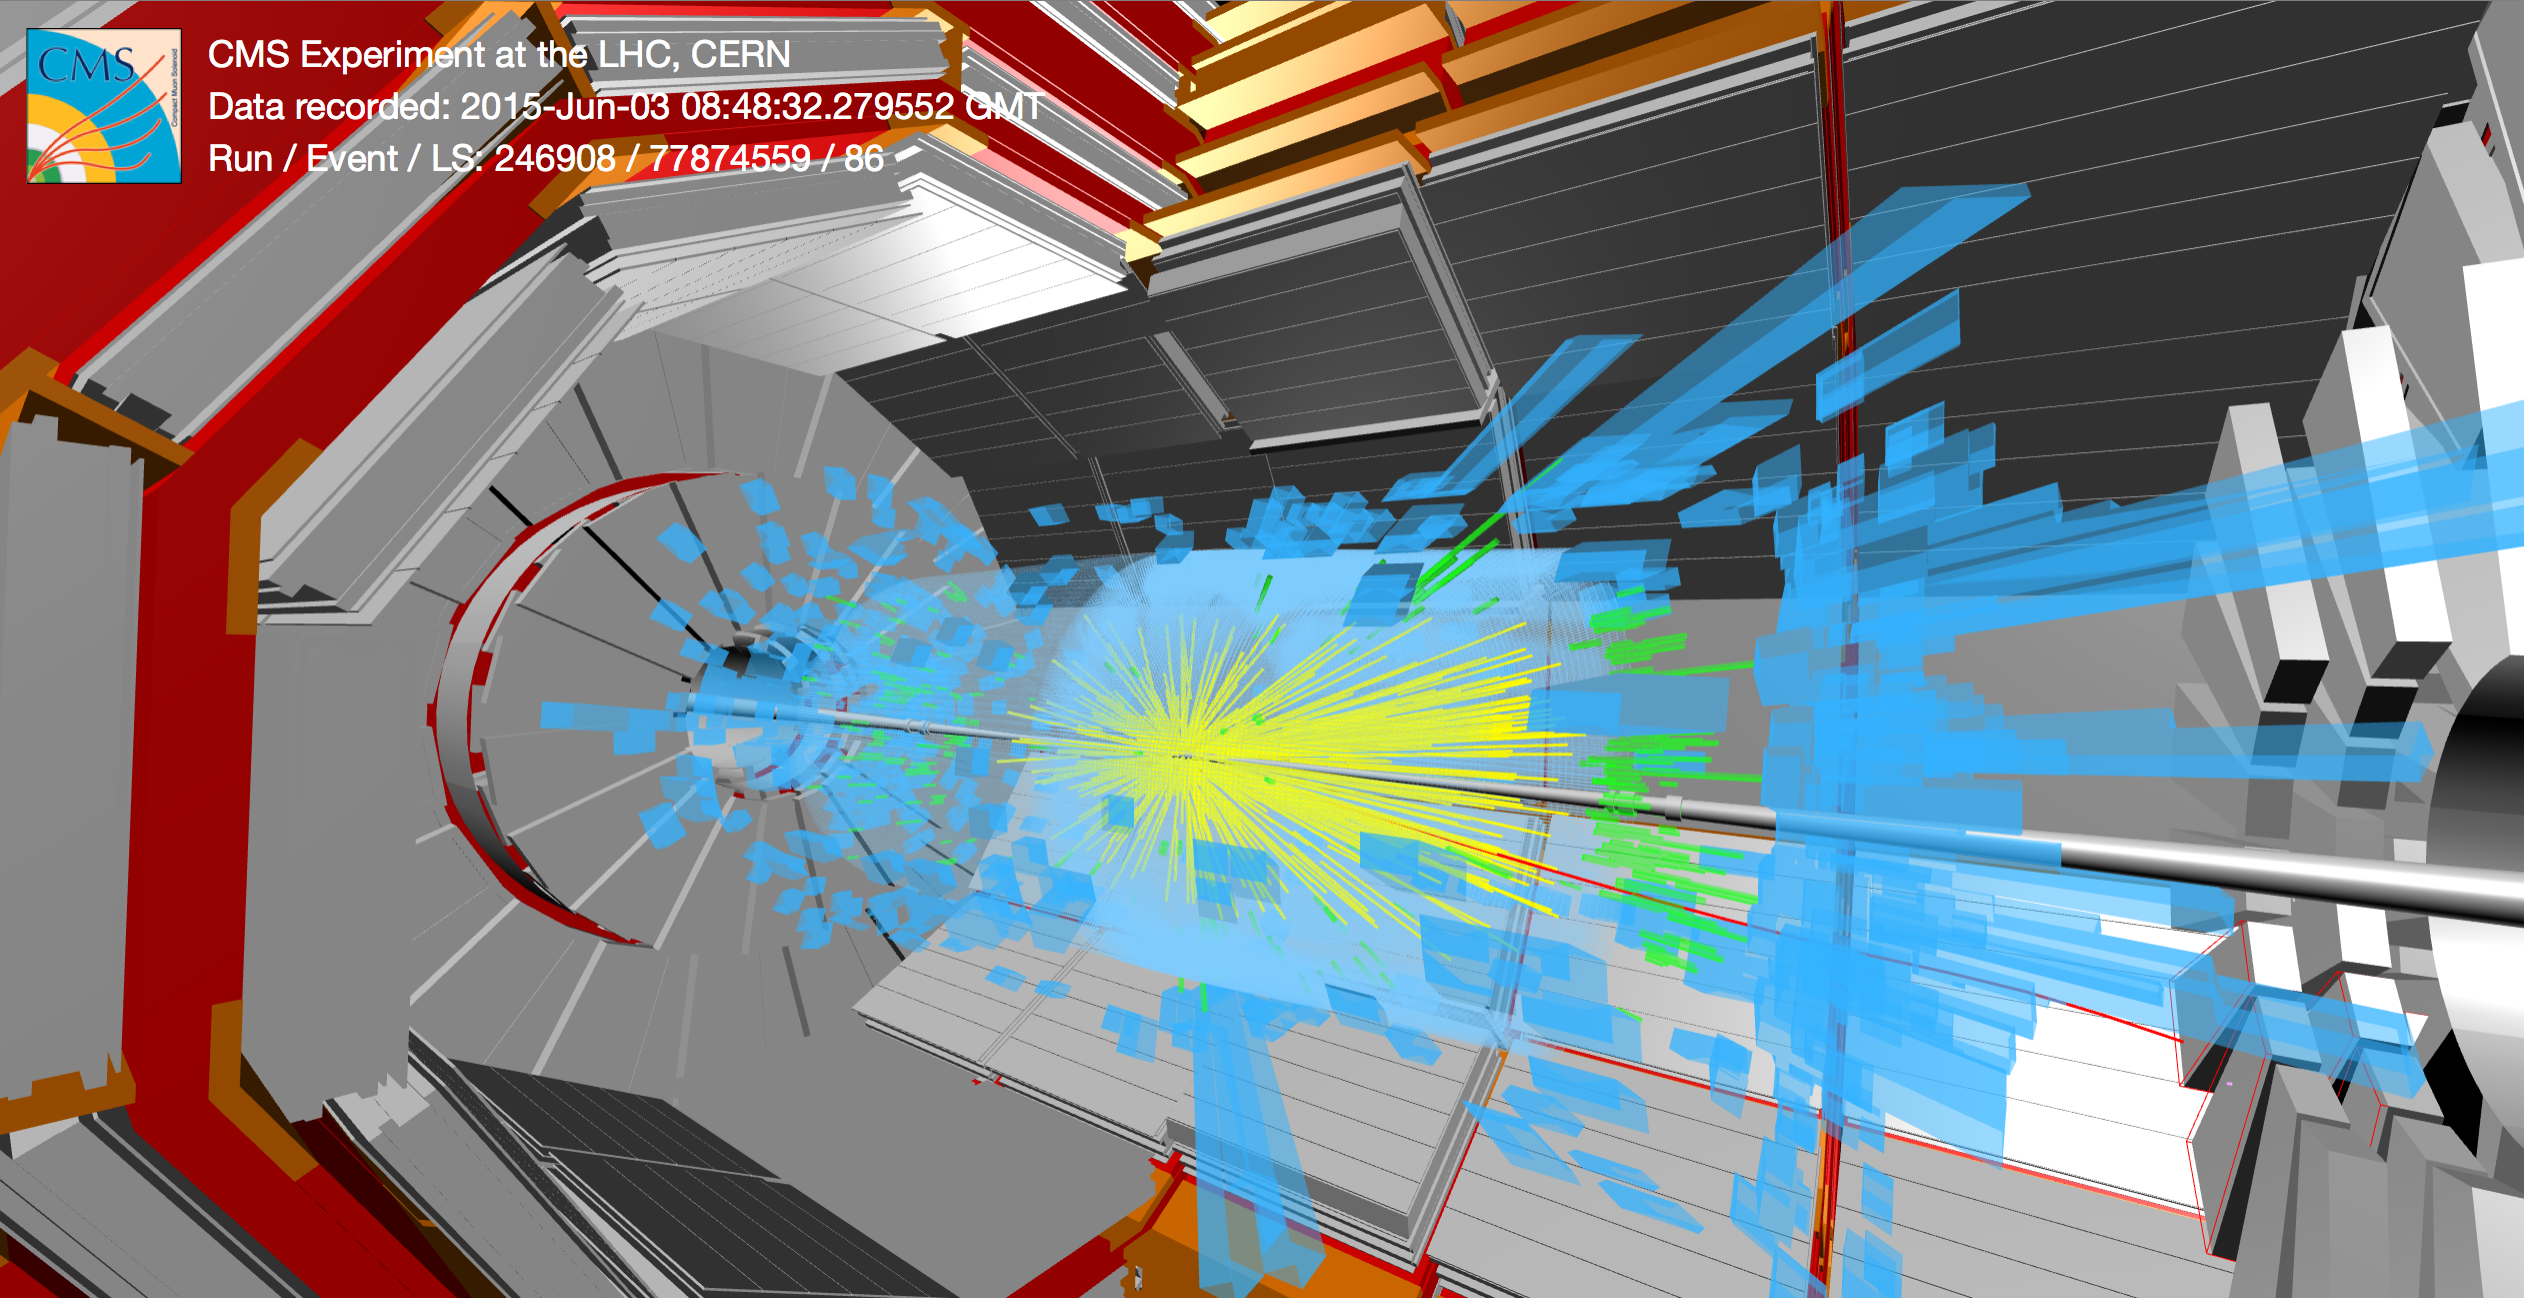
\includegraphics[scale=0.1]{exemplo_de_figura}
   \caption{Uma figura qualquer}
  \end{figure}
\end{frame}

\begin{frame}[fragile]{Inserindo mais de uma figura}

Podemos adicionar mais de uma figura no mesmo ambiente ao utilizar o comando \verb|\includegraphics[tamanho]{nomedafigura}|. Porém, temos que ter cuidado com os tamanhos das figuras e as posições.
\begin{itemize}
\item Figura lado a lado: incluir os comandos \verb|\includegraphics[]{}| um em baixo do outro
\item Figura em cima e embaixo: incluir os comandos \verb|\includegraphics[]{}| separados por \verb| \\ |
\end{itemize}

\end{frame}

\begin{frame}[fragile]{Exemplo - Figura lado a lado}
 \verb| \begin{figure}[h] |\\
       \verb| \centering |\\
       \verb| 
\includegraphics[scale=0.1]{furg.png} |\\
       \verb| 
\includegraphics[scale=0.1]{imef.jpg} |\\
       \verb|\caption{Exemplo:lado a lado}| \\
       \verb| \end{figure} |
\begin{figure}
\centering

\includegraphics[scale=0.1]{furg.png}

\includegraphics[scale=0.1]{imef.jpg}
\caption{Exemplo:lado a lado}
\end{figure}
\end{frame}


\begin{frame}[fragile]{Exemplo - Figura em cima e embaixo}
\begin{columns}
\begin{column}{0.5\textwidth}
\scriptsize
 \verb| \begin{figure}[h] |\\
       \verb| \centering |\\
       \verb| 
\includegraphics[scale=0.1]{furg.png} \\ |\\
       \verb| 
\includegraphics[scale=0.1]{imef.jpg} |\\
       \verb|\caption{Exemplo: em cima e embaixo}|\\
       \verb| \end{figure} |

\end{column}

\begin{column}{0.5\textwidth}
\begin{figure}
\centering

\includegraphics[scale=0.1]{furg.png} \\

\includegraphics[scale=0.1]{imef.jpg}
\caption{Exemplo: em cima e embaixo}
\end{figure}
\end{column}
\end{columns}
\end{frame}

\begin{frame}[fragile]{Inserindo figuras com subtítulos}

Para ter um controle de títulos e subtítulos de figuras devemos utilizar o ambiente \texttt{subfigure} e o pacote \texttt{subcaption} no preambulo.

\begin{figure}
\centering
\begin{subfigure}{0.5\textwidth}
\centering

\includegraphics[scale=0.1]{furg.png}
\caption{FURG}
\end{subfigure}%
\begin{subfigure}{0.5\textwidth}
\centering

\includegraphics[scale=0.1]{imef.jpg}
\caption{IMEF}
\end{subfigure}
\caption{Exemplo de figuras com subtítulos}
\end{figure}

\end{frame}

\begin{frame}[fragile]{Inserindo figuras com subtítulos - Código}
\scriptsize
\begin{verbatim}
\usepackage{subcaption}
\end{verbatim}

\verb|\begin{figure}| \\
\verb|\centering| \\
\hspace{0.5cm}\verb|\begin{subfigure}{0.5\textwidth}| \\
\hspace{1cm}\verb|\centering| \\
\hspace{1cm}\verb|
\includegraphics[scale=0.1]{furg.png}| \\
\hspace{1cm}\verb|\caption{FURG}| \\
\hspace{0.5cm}\verb|\end{subfigure}%| \\
\hspace{0.5cm}\verb|\begin{subfigure}{0.5\textwidth}| \\
\hspace{1cm}\verb|\centering| \\
\hspace{1cm}\verb|
\includegraphics[scale=0.1]{imef.jpg}| \\
\hspace{1cm}\verb|\caption{IMEF}| \\
\hspace{0.5cm}\verb|\end{subfigure}| \\
\verb|\caption{Exemplo de figuras com subtítulos}| \\
\verb|\end{figure}| \\
\end{frame}

\subsection{Referenciando}

\begin{frame}[fragile]{Lidando com referências}
Uma das grandes vantagens do \LaTeX \ é a facilidade de fazer referências a figuras, tabelas, equações, artigos, livros, etc.. 
\\
Para citar alguma figura, tabela ou equação, devemos adicionar o comando,

\begin{center}
\verb|\label{nome}| 
\end{center}

em que \texttt{nome} será utilizado para a citação.
\\
Para chamar no texto, devemos utilizar o comando, 

\begin{center}
\verb|\ref{nome}|
\end{center}

\end{frame}

\begin{frame}{Lidando com referências - Exemplo}


\begin{equation}
\nabla \cdot \vec{E} = \frac{Q}{\varepsilon_0} \label{maxwell}
\end{equation}

\begin{figure}
\centering

\includegraphics[scale=0.05]{furg.png}
\caption{Logo FURG}
\label{furg}
\end{figure}


A equação \ref{maxwell} é a primeira equação de Maxwell. A figura \ref{furg} é o logo da FURG

\end{frame}

\begin{frame}[fragile]{Lidando com referências - Código do Exemplo}
\small
\verb|\begin{equation}|\\
\verb|\nabla \cdot \vec{E} = \frac{Q}{\varepsilon_0} \label{maxwell}|\\
\verb|\end{equation}|\\
\vspace{0.2cm}
\verb|\begin{figure}|\\
\hspace{0.5cm}\verb|\centering|\\
\hspace{0.5cm}\verb|
\includegraphics[scale=0.05]{furg.png}|\\
\hspace{0.5cm}\verb|\caption{Logo FURG}| \\
\hspace{0.5cm}\verb|\label{furg}| \\
\verb|\end{figure}| \\
\vspace{0.2cm}
\verb|A equação \ref{maxwell} é a primeira equação de Maxwell.|
\verb| A figura \ref{furg} é o logo da FURG|
\end{frame}

\section{Módulo III}

\begin{frame}
\begin{center}
 {\Huge  Módulo III}
 \\
 {\normalsize Beamers e Personalizações}
\end{center}
\end{frame}

\subsection{Apresentações $Beamer$}

\subsubsection{Estrutura}

\begin{frame}[fragile]{Estrutura}
\begin{itemize}
  \item Em \LaTeX\ é possível criar apresentações de uma forma simples e de qualidade, com o pacote \verb| beamer |. Basta definir como classe:\\
  \begin{center}
  \verb| \documentclass[opções]{beamer} |
  \end{center}
  \item algumas opções são tamanho \verb|8pt,9pt,10pt,11pt,...|;
  \item o uso de pacotes é idêntico às outras classes \verb| book, article | etc.;
  \item informações básicas sobre o documento são:\\
  \verb| \title{}|\\
  \verb|\subtitle{}|\\
  \verb|\date[]{}|\\
  \verb|\author{}|\\
  \verb|\institute{}|\\
  \verb|\logo{}|
\end{itemize}
\end{frame}


\begin{frame}[fragile]{Estrutura}{Corpo}

\begin{itemize}
 \item da mesma forma que outras classes, tudo o que estiver entre 
    \begin{center}
     \verb| \begin{document} |\\
      .\\
      .\\
      .\\
     \verb| \end{document} |
    \end{center}
constitui-rá tudo o que estiver escrito nos \emph{frames}: textos, listas, tabelas, figuras, equações etc;
\item um frame é uma página da apresentação, e é construído por:\\
\verb|\begin{frame}[opções]{título}{subtítulo}|\\
\verb|\end{frame}|
\end{itemize}
\end{frame}

\begin{frame}[fragile,b]{Estrutura}{Corpo}
\begin{itemize}
\item para se criar o sumário da apresentação, cria-se um frame com o comando \verb|\tableofcontents|:\\
\verb|\begin{frame}{Sumário}|\\
\verb|\tableofcontents|\\
\verb|\end{frame}|
\item se caso o sumário for muito grande e não couber no frame, crie duas colunas (a seguir) ou use o comando \verb|{\fontsize{10pt}{10.0}\selectfont todo o frame aqui }|
e ajuste a fonte (primeiro \verb|{}| ) o espaçamento de linhas (segundo \verb|{}|) até ajustar o sumário,
\item exemplo de opções: 
\begin{itemize}
   \item  \verb|fragile|, usado para \emph{macros}, como o \verb|verbatim|;\\
   \item \verb|b|, \verb|c| ou \verb|t|, posição do texto no frame (\verb|b| este frame); 
    \end{itemize}
 \end{itemize}

\end{frame}


\subsubsection{Ambientes}


\begin{frame}[fragile]{Ambientes}{Blocos e Colunas}
\begin{itemize}
 \item ambientes muito utilizados nos beamers são: \verb|itemize|, \verb|enumerate|, \verb|description|;
 \item outros ambientes são os \verb|blocos|: \verb|block|, \verb|alertblock|, \verb|exampleblock|, ...
\end{itemize}
\begin{block}{Nome do Bloco}

\begin{verbatim}
\begin{block}{Nome do Bloco}
. . . 
\end{block}
\end{verbatim}

\end{block}

\begin{alertblock}{Um Alerta!}

\begin{verbatim}
\begin{alertblock}{Um Alerta!}
. . .
\end{alertblock}
\end{verbatim}

\end{alertblock}


\end{frame}


\begin{frame}[fragile]{Ambientes}{Blocos e Colunas}
\begin{itemize}
\item dividir um frame em colunas pode ser bastante útil;
\item para criá-las basta usar:
%
\begin{columns}
\begin{column}{5cm}
	
\begin{verbatim}
\begin{columns}
\begin{column}[t]{tamanho}
Criando colunas.
Duas colunas.
\end{column}
\end{verbatim}

\end{column}
    
\begin{column}{5cm}
    
\begin{verbatim}     
\begin{column}[t]{tamanho}
Tamanho define a largura 
das colunas. 
\end{column}
\end{columns}
\end{verbatim}

\end{column}

\end{columns}
\item em uma coluna podemos ter um texto e na outra uma figura (exercício).
\end{itemize}
\end{frame}



\begin{frame}[fragile]{Ambientes}{Pause e Overlays}
\begin{itemize}
 \item o comando \verb|pause| nos permite pausar os tópicos de ambientes como \verb|itemize|;
 \pause
 \item dando sequência nestes 
 \pause
 \item na medida que avançamos a apresentação;
 \pause
\end{itemize}

\begin{verbatim}
\begin{itemize}
 \item o comando \verb|pause| nos permite pausar os tópicos de 
 ambientes como \verb|itemize|;
 \pause
 \item dando sequência nestes 
 \pause
 \item na medida que avançamos a apresentação;
 \pause
\end{itemize}
\end{verbatim}

\end{frame}


\begin{frame}[fragile]{Ambientes}{Pause e Overlays}
\begin{itemize}
 \item os \verb|overlays| são utilizados quando queremos usar "muitos pauses",
 \item se não quisermos repetir a todo o momento o comendo \verb|pause|, basta introduzir \verb|[<+->]| de pois de \verb|{itemize}|
 \item o ambiente \verb|itemize| do frame anterior fica
\end{itemize}

\begin{verbatim}
 \begin{itemize}[<+->]
 \item o comando \verb|pause| nos permite pausar os tópicos de 
 ambientes como \verb|itemize|;
 \item dando sequência nestes 
 \item na medida que avançamos a apresentação;
\end{itemize}
\end{verbatim}

\end{frame}



\begin{frame}[fragile]{Ambientes}{Exercício}
\begin{columns}

\begin{column}[t]{6cm}
\begin{figure}[b]
\centering
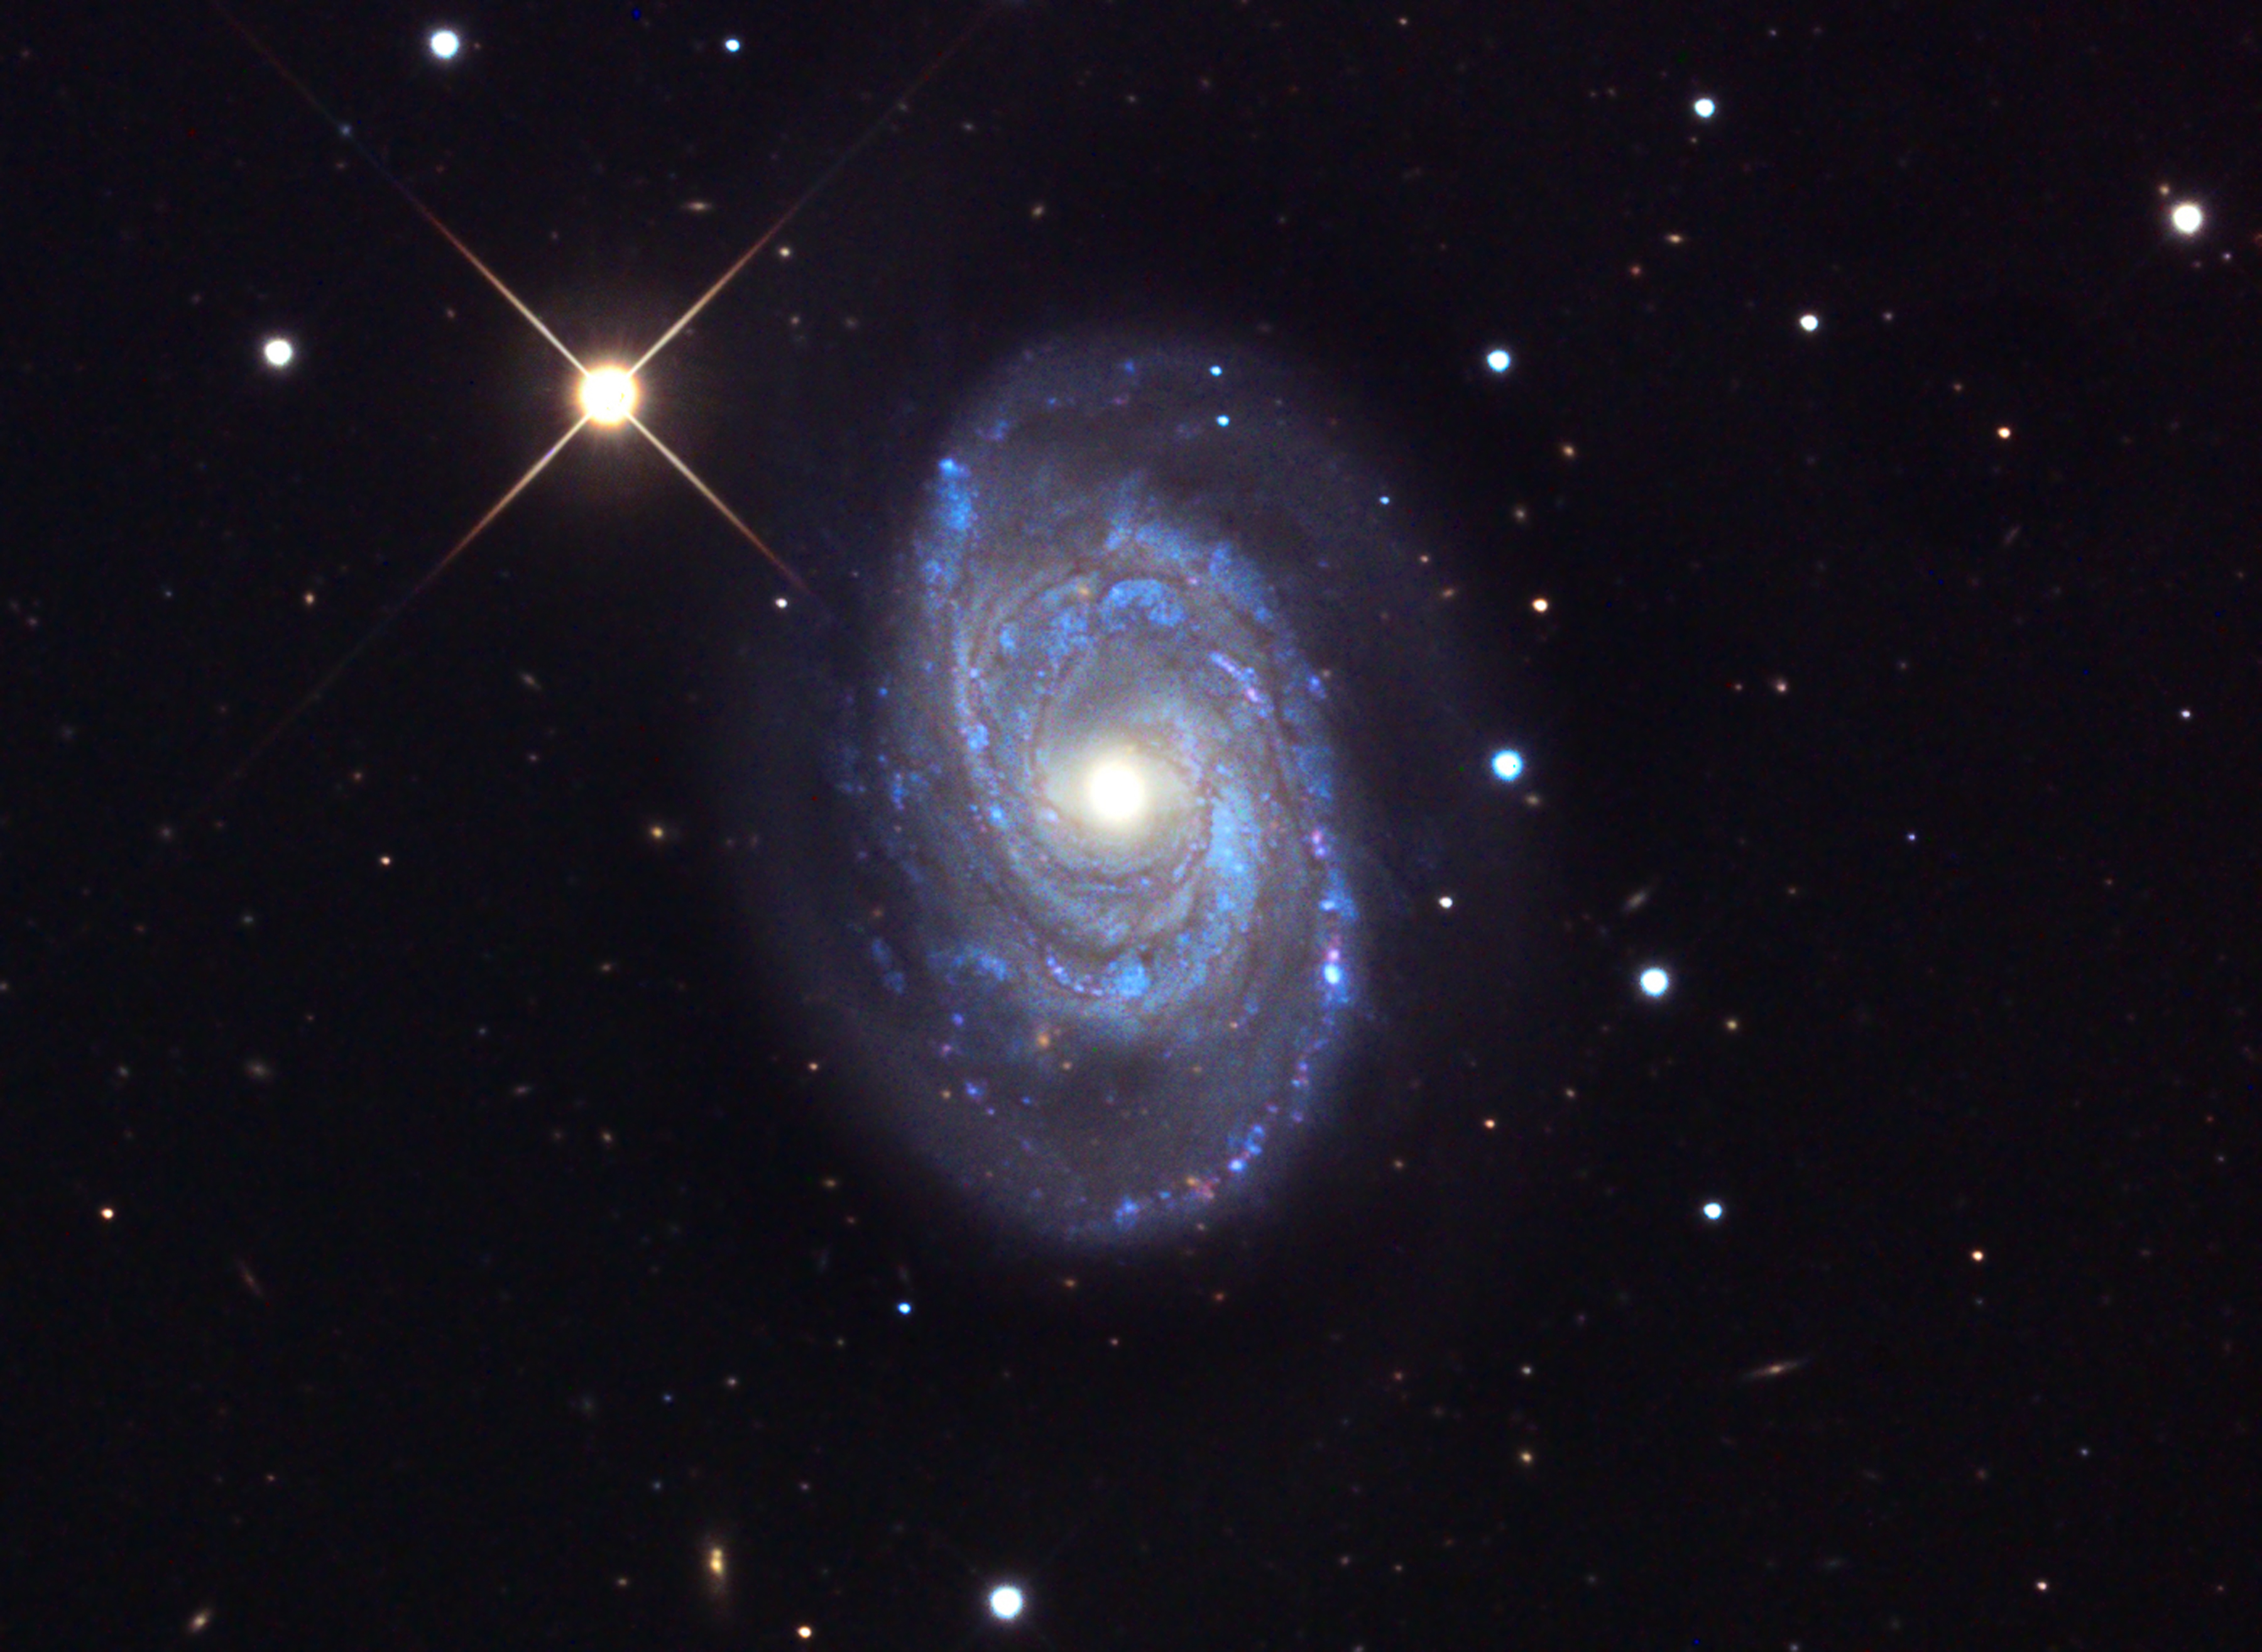
\includegraphics[scale=0.18]{NGC_5371.jpg}
\caption{NGC 5371}
\label{mod_3_ex_1}
\end{figure}
algum texto algum texto
algum texto algum texto
\end{column}


\begin{column}[t]{6cm}

\begin{block}{Exercício}
Crie um frame idêntico a este.
Use \verb|\setbeamercovered{transparent}| para itens com pauses ficarem "sombreados".
\end{block}

\begin{itemize}[<+->]
 \item crie duas colunas com 6cm cada;
 \item insira uma figura na coluna esquerda; 
 \item crie um bloco;
 \item e para os itens, use \verb|overlays|;
\end{itemize}

\end{column}

\end{columns}

\end{frame}


\subsubsection{Temas}

\begin{frame}[fragile]{Temas}{Temas, Cor, Fonte}
 \begin{itemize}
  \item vários modelos de \emph{beamers} estão disponíveis para utilização;
  \item para isso, modificamos o tema com:\\
  \verb|\usetheme{}| - modifica a estrutura do tema;\\
  \verb|\usecolortheme{}| - modifica a cor do tema;\\
  \verb|\usefonttheme{}| - modifica a fonte do tema
  \item exemplos destes temas são: \verb|\usetheme{Darmstadt}|, \verb|\usecolortheme{orchid}|, \verb|\usefonttheme{serif}| (utilizados nesta apresentação);
 \end{itemize}
\end{frame}


\begin{frame}{Temas}{Exemplos de Temas}
\begin{center}
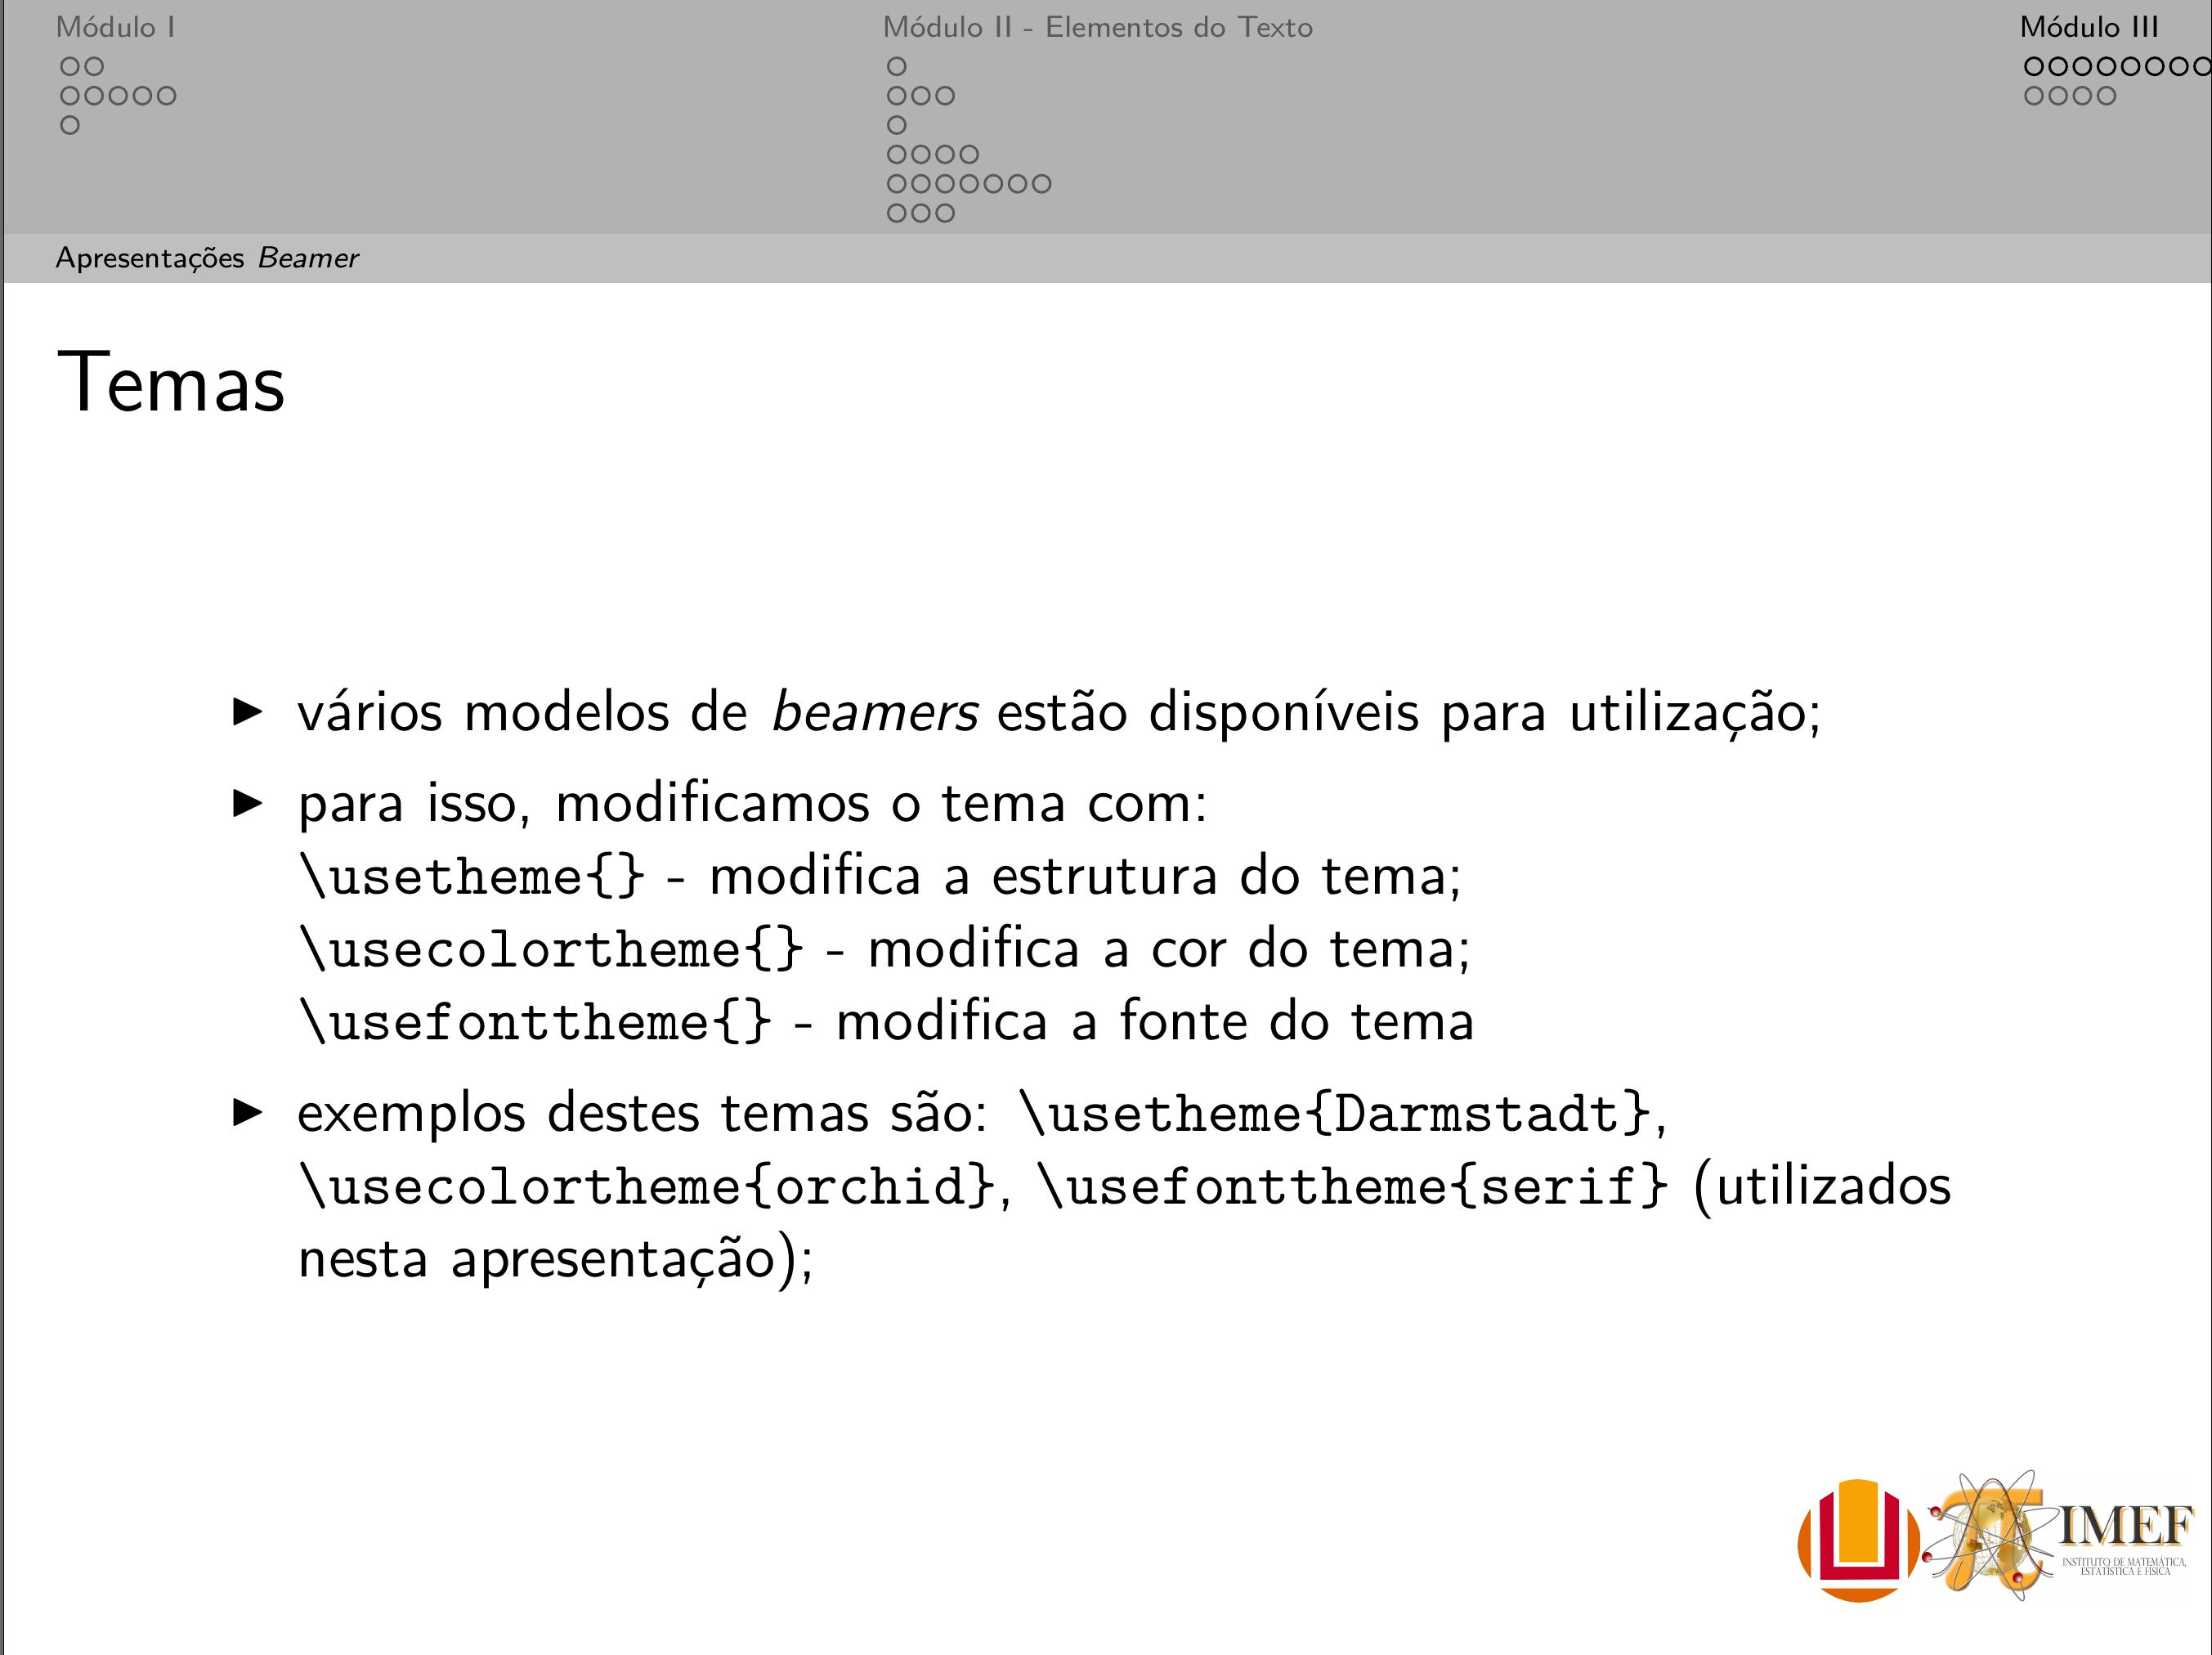
\includegraphics[width=0.40\textwidth]{beamer_sze_seau.jpg}
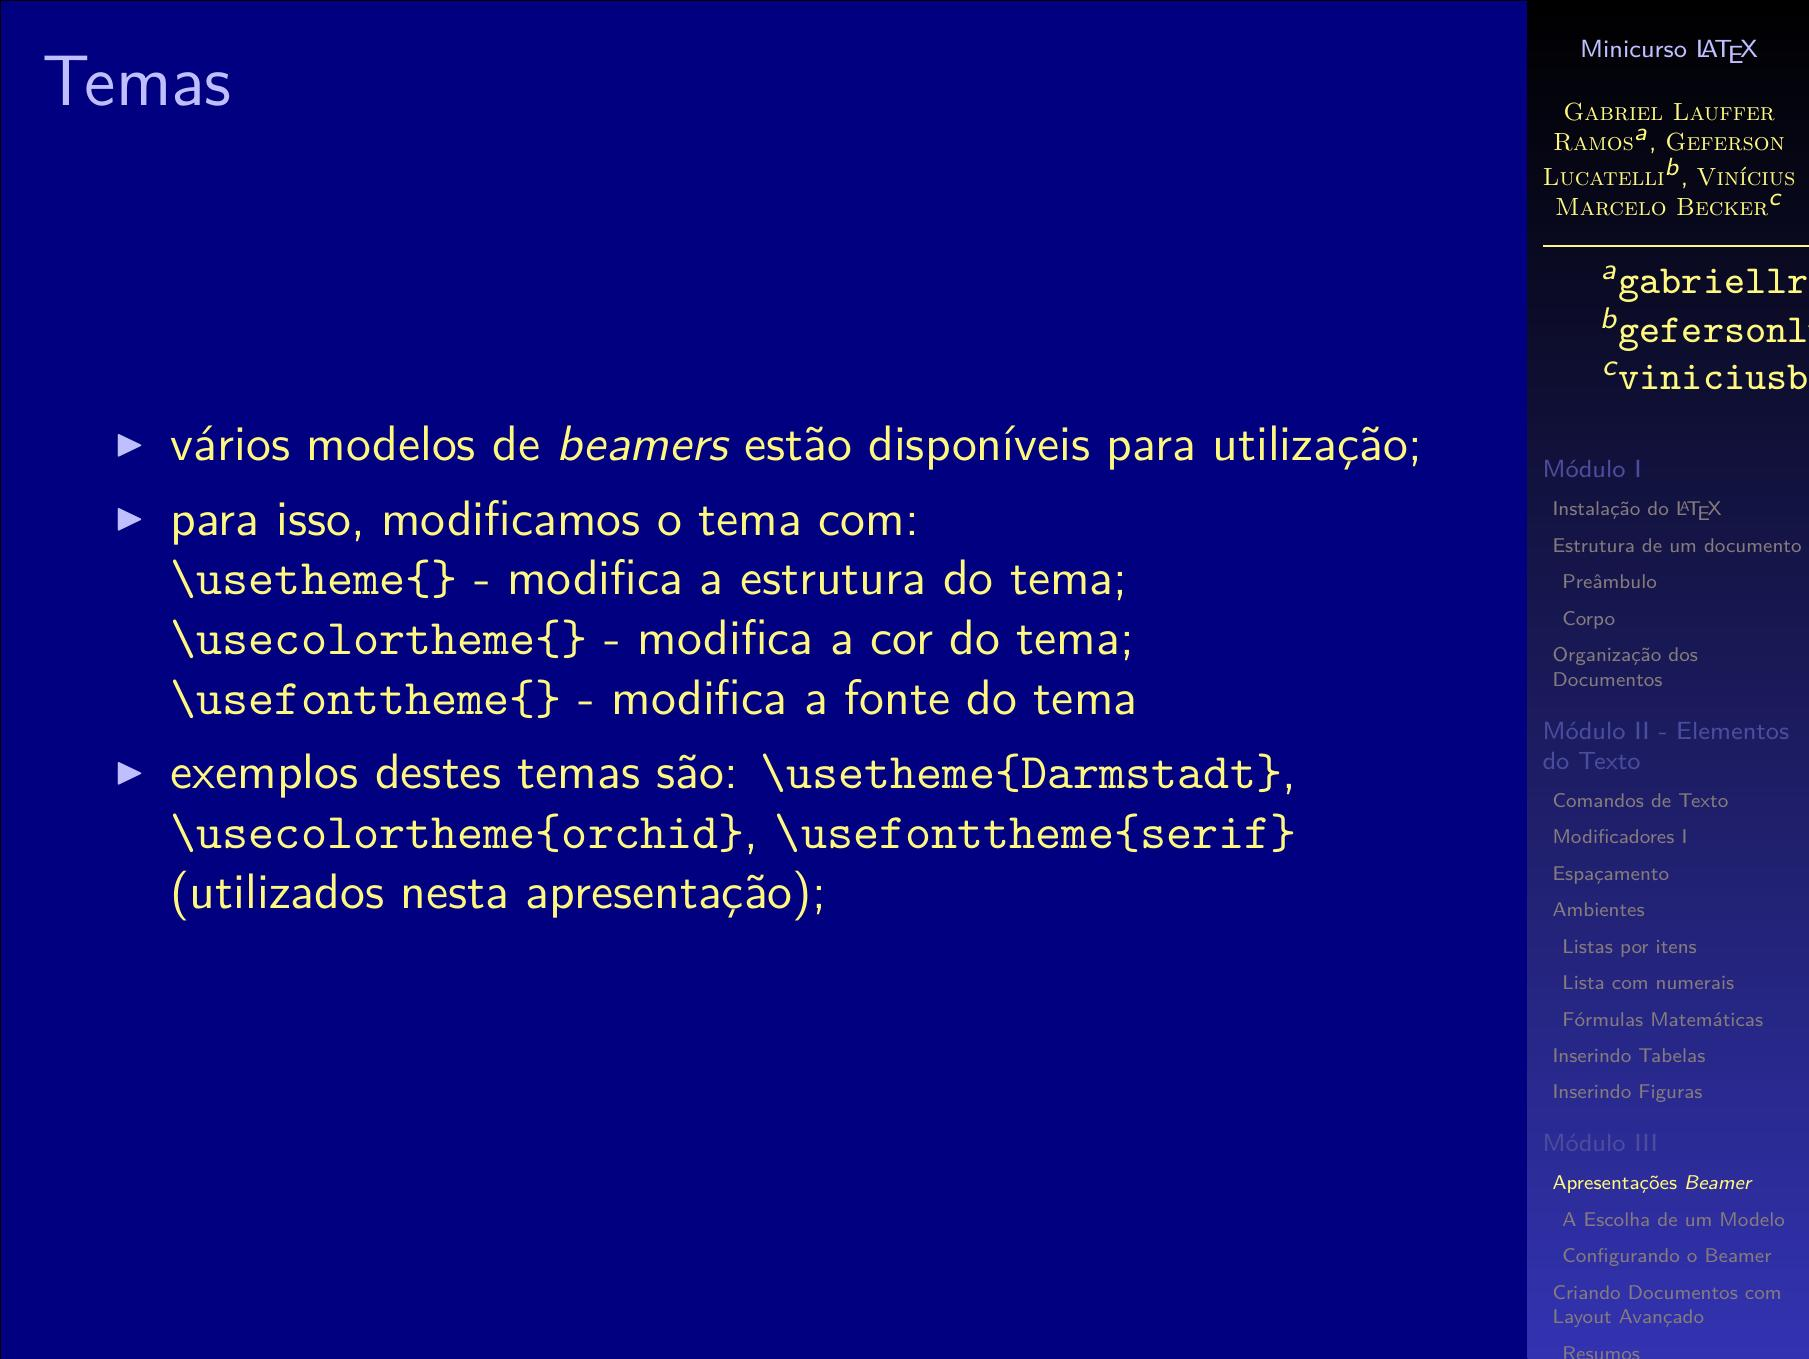
\includegraphics[width=0.40\textwidth]{beamer_marb_alb.jpg}\\
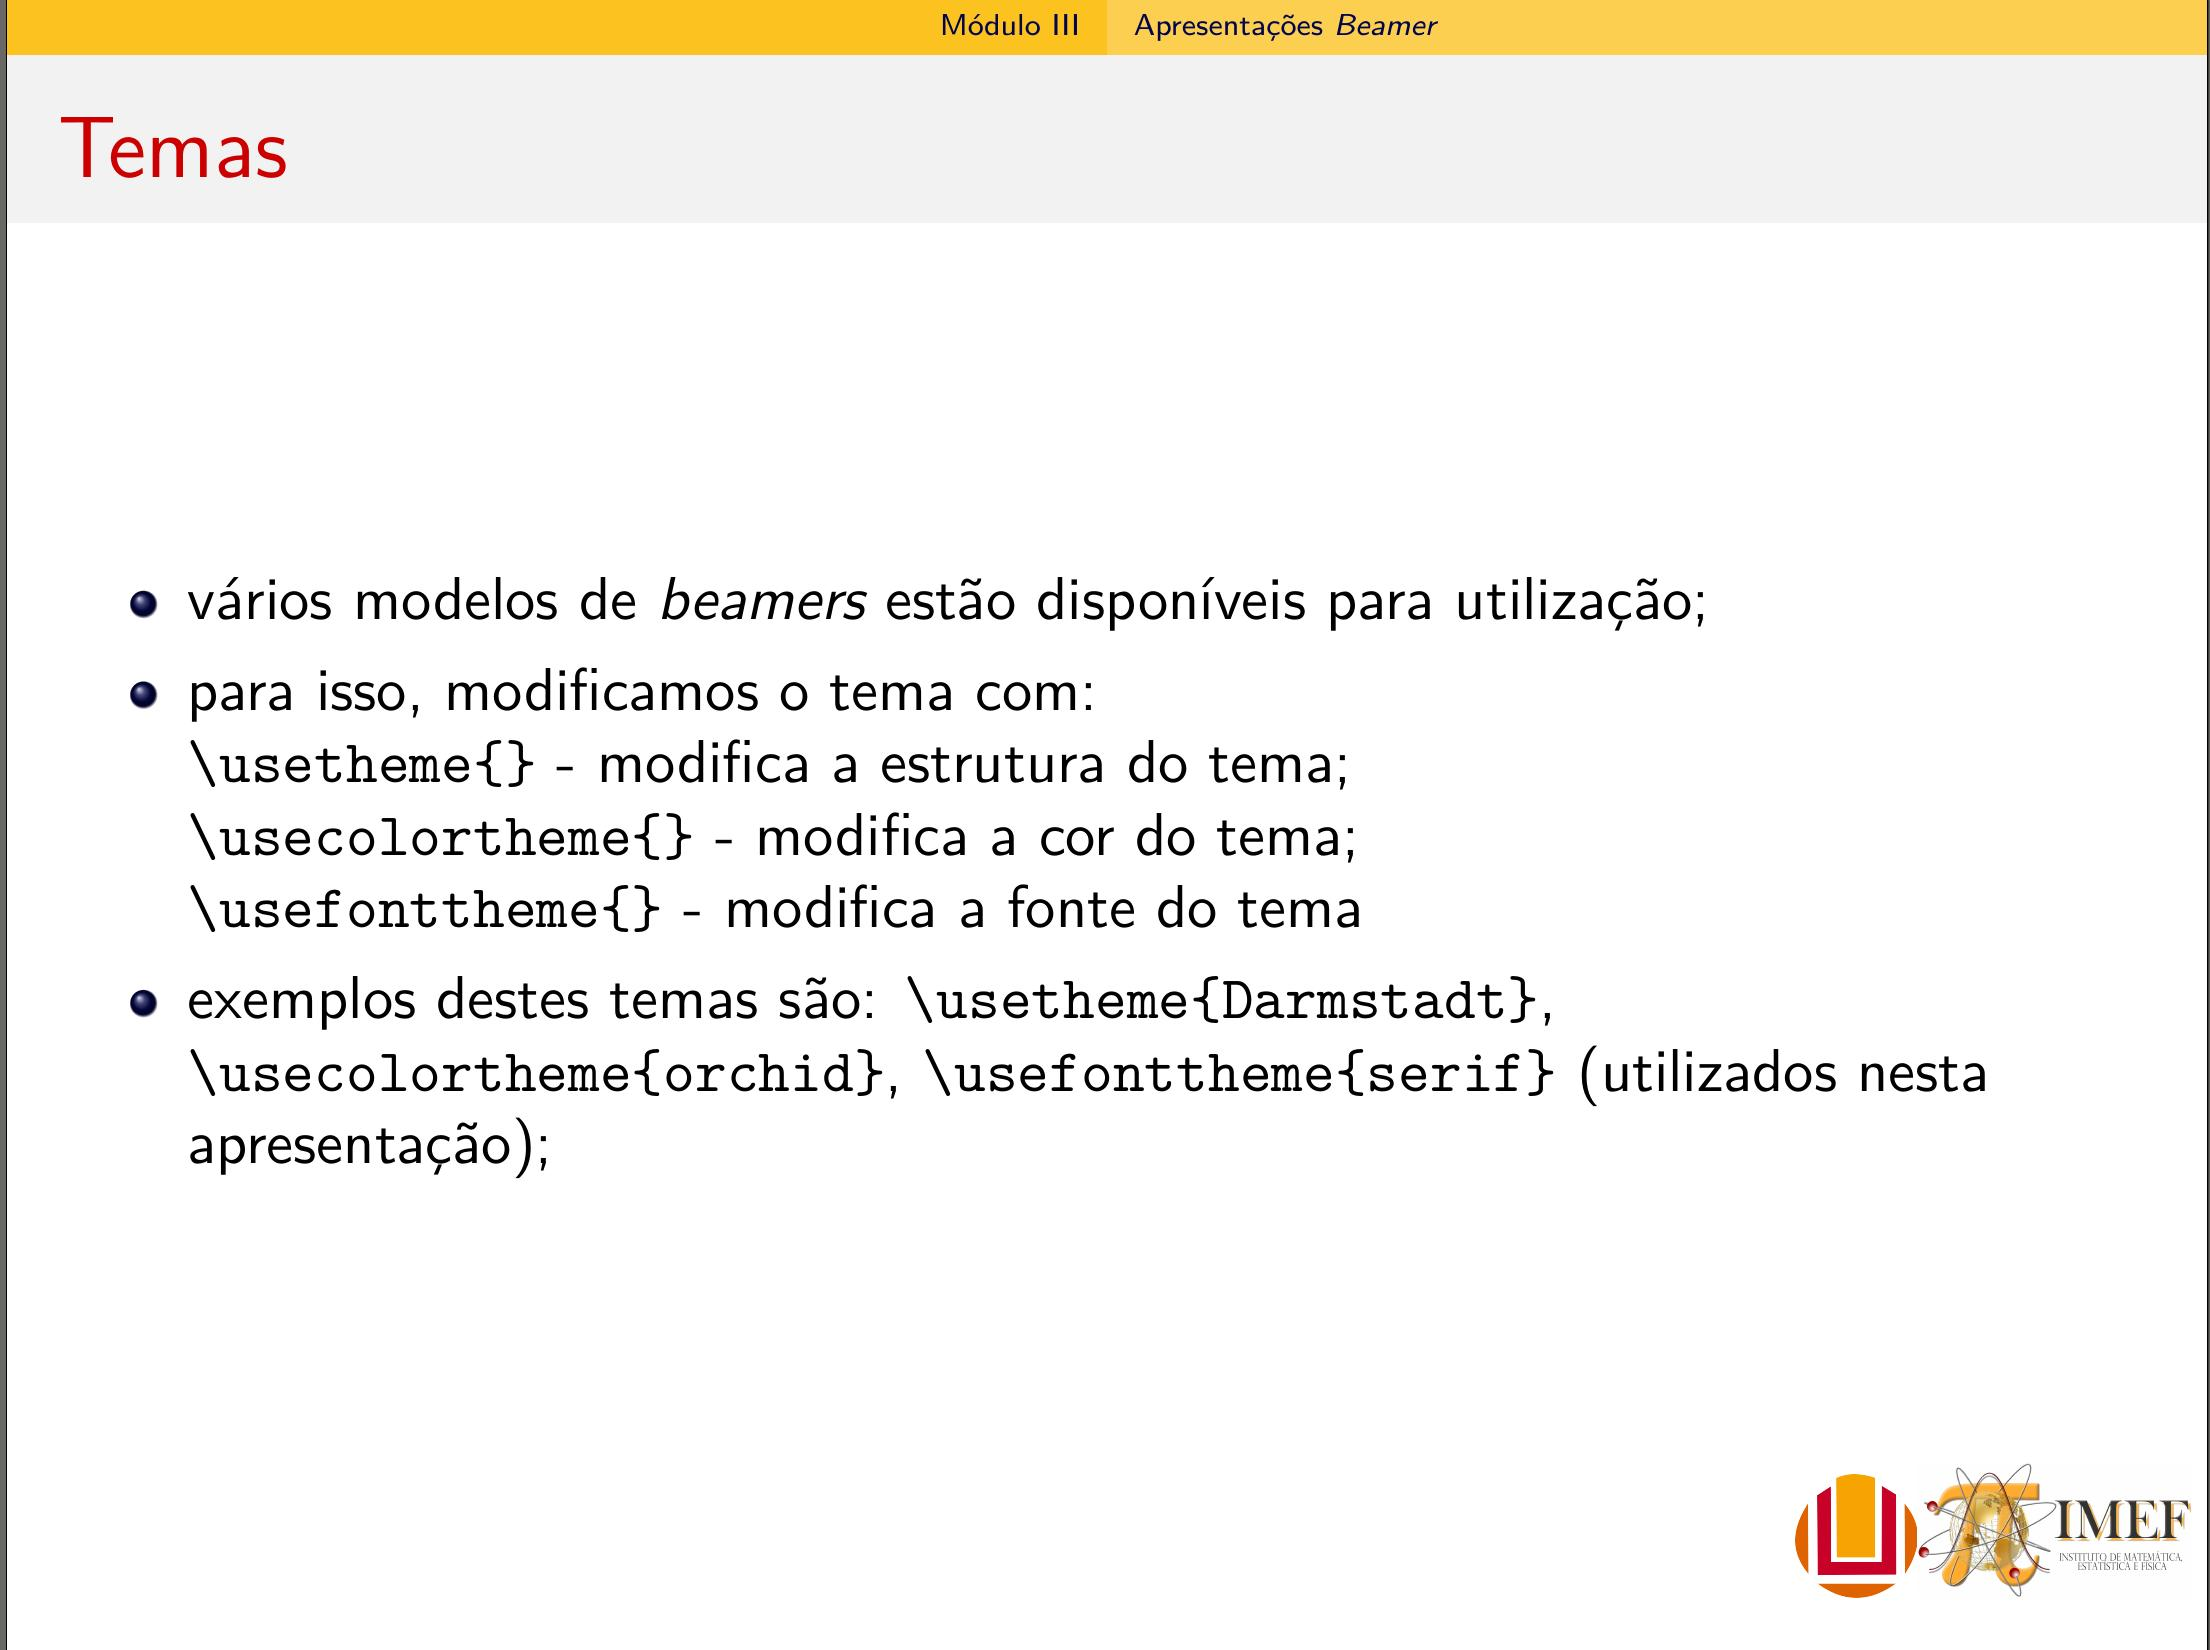
\includegraphics[width=0.40\textwidth]{beamer_cambr_crane.jpg}
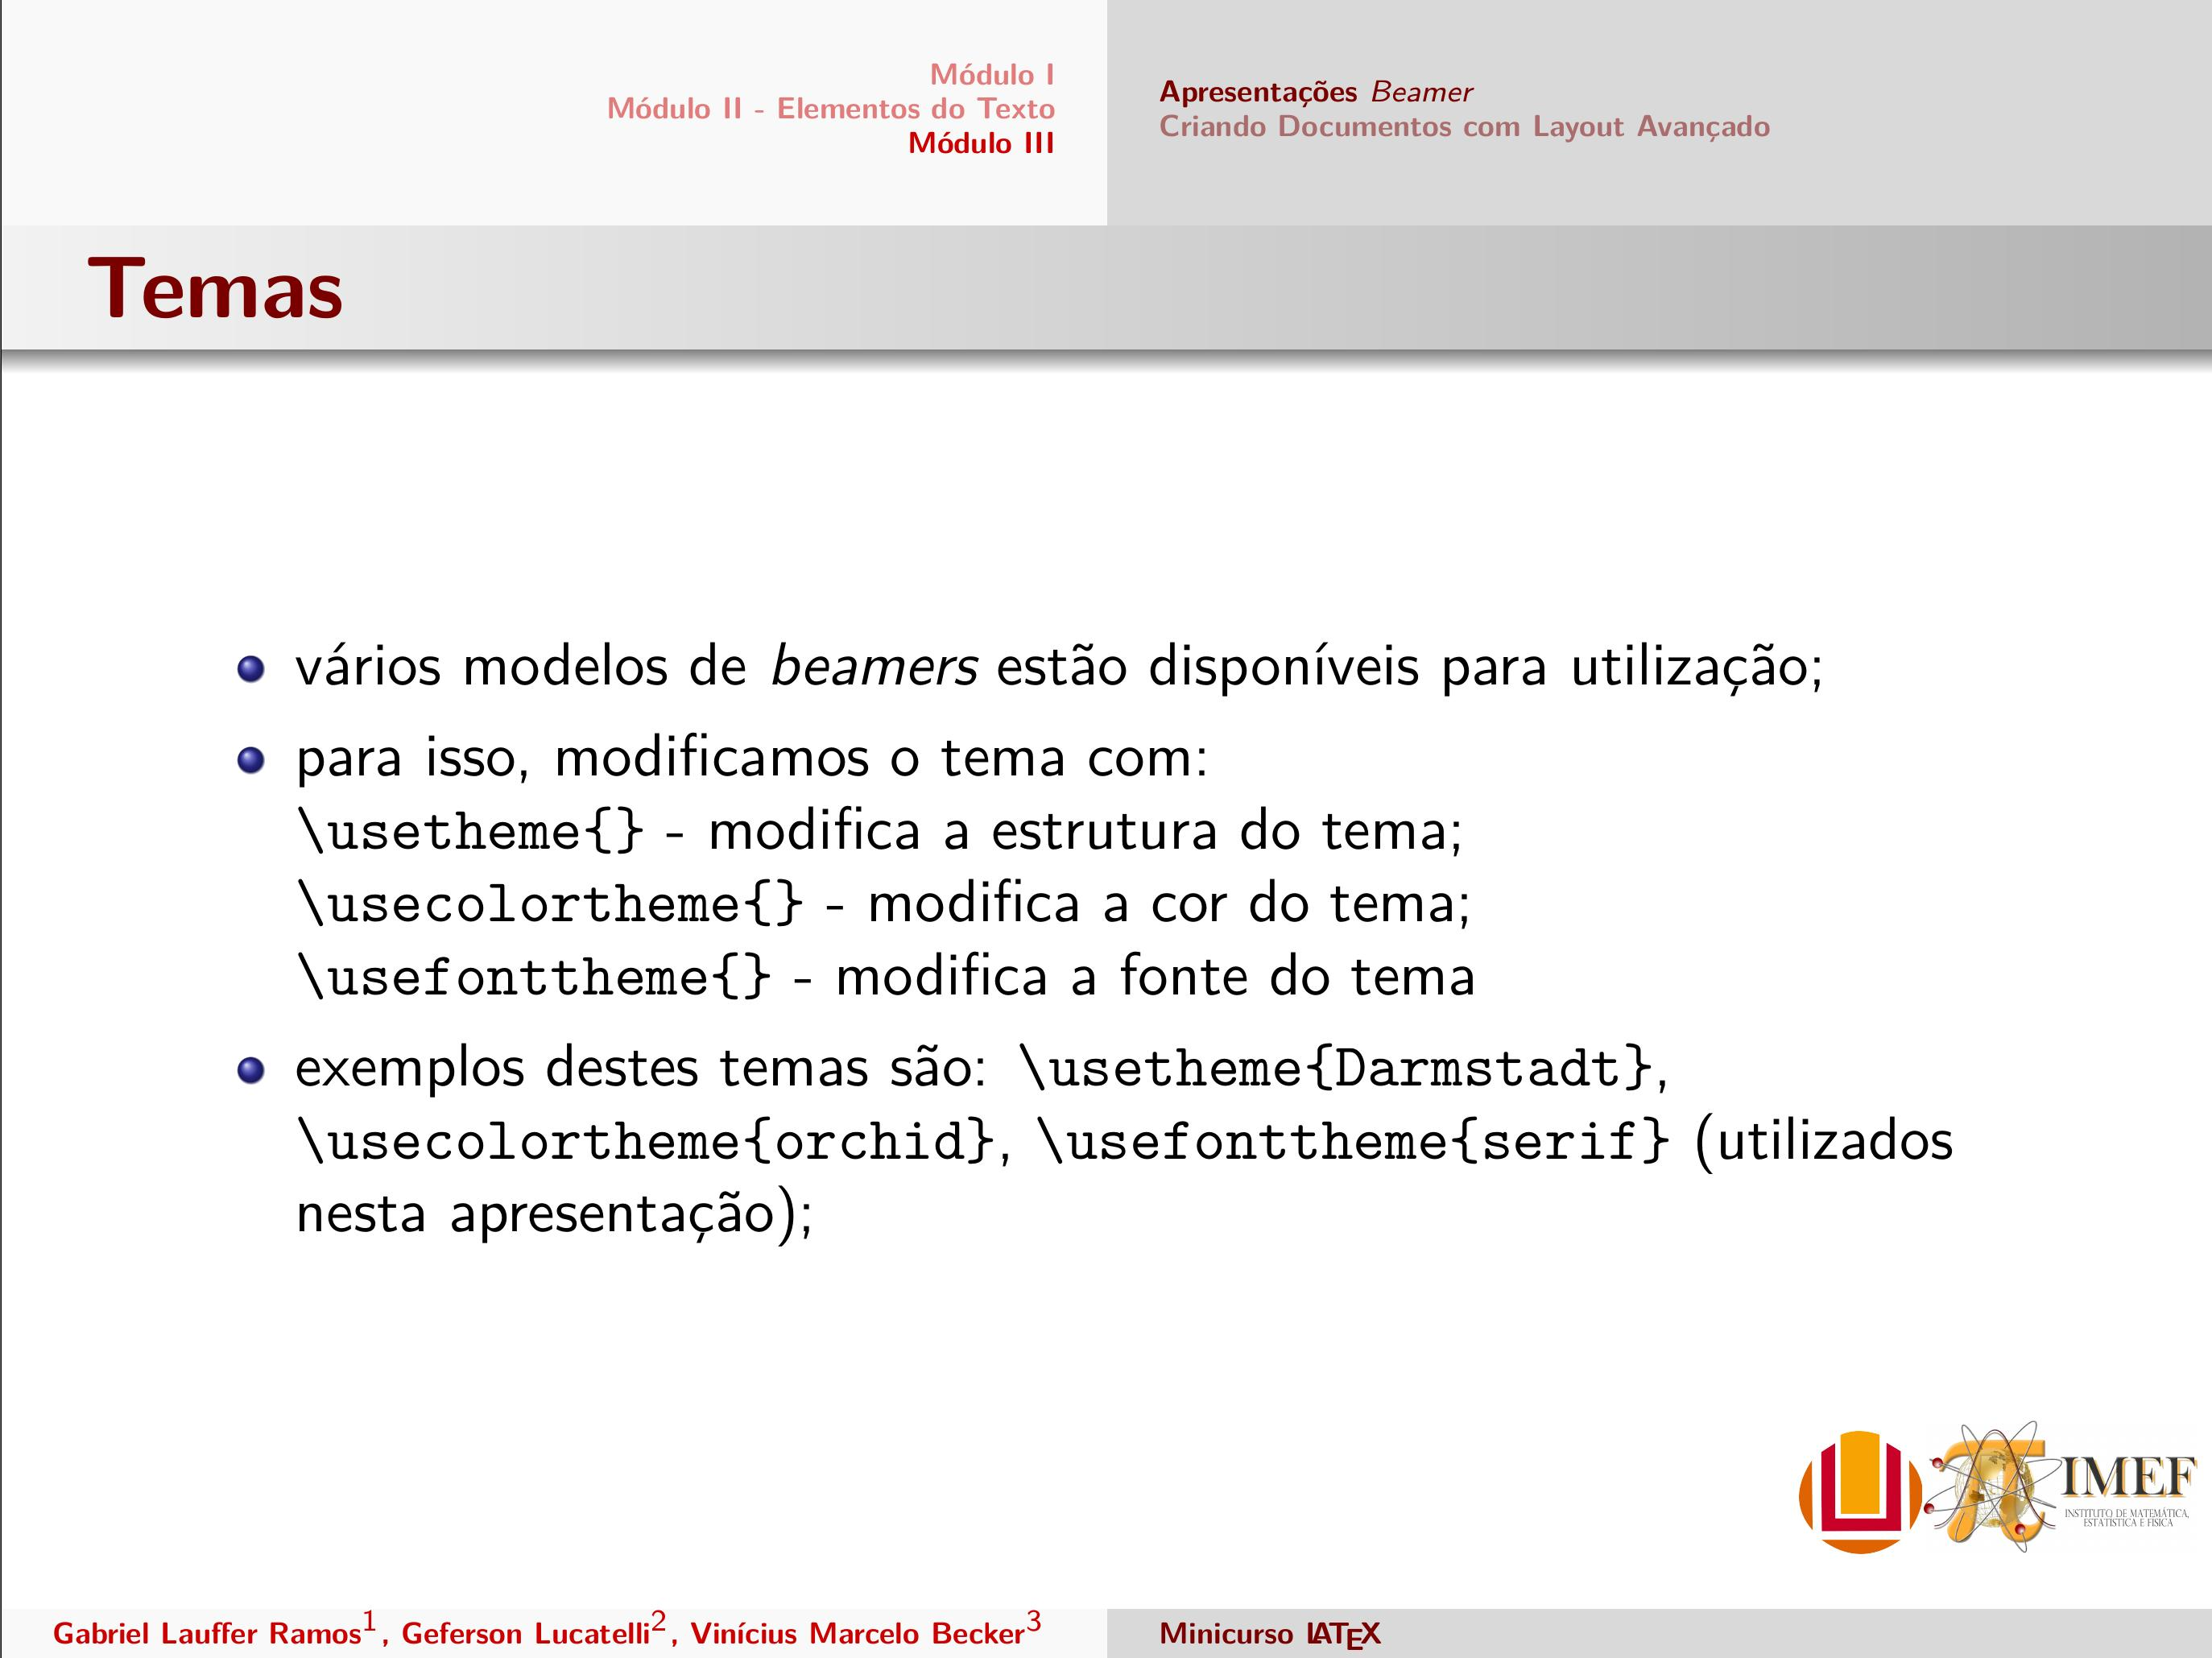
\includegraphics[width=0.40\textwidth]{beamer_beav_war.jpg}
\captionof{figure}{}
\end{center}
\end{frame}


\begin{frame}[fragile]{Temas}{Exemplo}
\begin{exampleblock}{Exemplo - Este Beamer}
{\fontsize{6pt}{6.0}\selectfont
\begin{verbatim}
\documentclass[10pt]{beamer}
\mode<presentation>
{
  \usetheme{Darmstadt}
  \usecolortheme{orchid}
  \usefonttheme{serif}
  \setbeamertemplate{navigation symbols}{}
  \setbeamertemplate{caption}[numbered]
  \setbeamercovered{transparent}
  \setbeamertemplate{footline}
}
\usepackage[brazil]{babel}
\usepackage{lmodern}
\usepackage[utf8x]{inputenc}

\title{Minicurso \LaTeX}
\subtitle{Semana Acadêmica da Física - FURG}
\date[2016]{Rio Grande, RS}
\author{
\textsc{Gabriel Lauffer Ramos}\inst{1}\footnote[1]{\texttt{gabriellramos@gmail.com}},
\textsc{Geferson Lucatelli}\inst{1}\footnote[2]{\texttt{gefersonlucatelli@furg.br}},
\textsc{Vinícius Marcelo Becker}\inst{1}\footnote[3]{\texttt{viniciusbecker@furg.br}}
}
\institute[IMEF]{{\large{Universidade Federal do Rio Grande}}\\
\inst{1}Instituto de Matemática, Estatística e Física}
\logo{

\includegraphics[scale=.10]{furg.png}

\includegraphics[scale=.08]{imef.jpg}
}
\end{verbatim}
}

\end{exampleblock}
\end{frame}

\subsection{Personalizando Documentos}

\begin{frame}[fragile]{Teses}
 \begin{itemize}
 \item com o \LaTeX\ é possível se criar inúmeros documentos, de variados estilos;
 \item vamos verificar primeiramente como construir um modelo de tese personalizada;
 \item mesmo sendo uma tese, usamos a classe \verb|book| com algumas opções:\\
 \verb|\documentclass[a4paper,10pt]{book}|
 \item usando o pacote \verb|geometry| podemos personalizar as margens do documento:\\
 \verb|\usepackage[a4paper,total={15.0cm,20.0cm}]{geometry}|
 \item o primeiro valor 15.0cm indica que 15.0cm serão usados para dispor o texto na 
 horizontal, e 20.0cm na vertical;
 \item para o papel a4, o limite máximo é \verb|total={21.0cm,29.7cm}|;
 \end{itemize}
\end{frame}


\begin{frame}[fragile]{Teses}{Capa e Título}
\begin{itemize}
 \item a estrutura é simples, e adicionamos elementos na medida que queremos;
 \item começaremos com a construção de uma capa;
 \item para isso usa-se o ambiente \verb|titlepage|:\\
 \verb|\begin{titlepage}|\\
 $\vdots$ \\
 \verb|\end{titlepage}|
 \item este deve estar no ambiente \verb|document|;
 \item no ambiente \verb|titlepage| informações que podem ser incluídas de imediado como já vimos são: \verb|\title{}|,  \verb|\author{}| e  \verb|\date{}|;
\end{itemize}
\end{frame}

\begin{frame}[fragile]{Teses}{Capa e Título}
 \begin{columns}
\begin{column}[t]{6cm}
 \begin{itemize}
  \item para incluir por exemplo o nome da Universidade, Instituto e outros elementos, iremos definir variáveis com o comando \verb|\newcommand|;
  \item vamos criar o comando \verb|\university{}|;
  \item a quantidade de argumentos é um, o nome da Universidade;
 \end{itemize}
\end{column}

\begin{column}[t]{6cm}
\begin{block}{Definindo Um Comando}
\begin{itemize}
\item usamos \verb|\newcommand{cmd}[args]{def}|;
 \item a variável \verb|cmd| é o nome do comando a ser chamado;
 \item \verb|args| é quantos argumentos estão atribuídos ao comando;
 \item \verb|def| é o que o comando irá fazer;
\end{itemize}

\end{block}
 
\end{column}

 
 \end{columns}

 
\end{frame}


\begin{frame}[fragile]{Teses}{Capa e Título}
\begin{itemize}
\item a definição para o novo comando será de nossa escolha; 
\item por exemplo, definir o nome da universidade com uma dada fonte, alinhamento etc;
\item podemos fazer
\end{itemize}
\begin{exampleblock}{Universidade}
{\fontsize{8pt}{6.0}\selectfont
\begin{verbatim}
\newcommand{\university}[1]
{
\begin{center}
\textsc{\LARGE #1} 
\end{center}
}
\end{verbatim}
}
\end{exampleblock}
\begin{itemize}
 \item \verb| #1| representa a seleção do argumento 1 para entrar no novo comando;
\end{itemize}

\end{frame}

\begin{frame}[fragile]{Teses}{Capa e Título}
\begin{itemize}
 \item podemos fazer o mesmo para o Instituto, mas vamos incluir dois argumentos;
 \item seja \verb|#1| o nome e \verb|#2| o website do instituto, então definindo \verb|\institute{}| como novo comando:
 \begin{exampleblock}{Instituto}
{\fontsize{8pt}{6.0}\selectfont
\begin{verbatim}
\newcommand{\institute}[2]
{
{\begin{center}
\textsc{\large #1}
\end{center}
}
{
\begin{center}
\small{\texttt{\url{ #2 }}}\vfill
\end{center}}}
\end{verbatim}
}
\end{exampleblock}
\end{itemize}

\end{frame}



\begin{frame}[fragile]{Teses}{Capa e Título}
\begin{itemize}
 \item um efeito pode ser adicionado para acomodar o título do trabalho com o instituto e universidade, por exemplo, linhas horizontais;
 \item definimos então: \verb|\newcommand{\linesH}[1]{\rule{\linewidth}{#1}}|, em que \verb|1#| é a grossura da linha;
 \item este comando produz:\\
 \linesH{0.01cm}
 \linesH{0.05cm}
 \linesH{0.1cm}
\end{itemize}

\end{frame}

\begin{frame}[fragile]{Teses}{Capa e Título}
\begin{itemize}
\item a definição \verb|\title{}| é está definida, mas se quisermos incluir o efeito da linha anterior no título, podemos redefinir 
o título com \verb|\renewcommand{cmd}[args]{def}|
\end{itemize}
\begin{exampleblock}{Título}
{\fontsize{8pt}{6.0}\selectfont
\begin{verbatim}
\renewcommand{\title}[1]{
\vspace*{\fill}
% \centering
\begin{center}
\lineH{0.1cm}
\Huge{{\bf #1 }}
\lineH{0.1cm}
\vspace*{\fill}
\end{center}
}
\end{verbatim}
}
\end{exampleblock}
\end{frame}



\begin{frame}[fragile]{Teses}{Capa e Título}
\begin{itemize}
 \item o \verb|\author{}| já é uma definição padrão, mas devemos redefini-la para usarmos no 
 ambiente \verb|\titlepage|;
 \item vamos incluir também a informação \verb|\supervisor{}|;
\end{itemize}

\begin{exampleblock}{Autor e Supervisor/Orientador}
{\fontsize{8pt}{6.0}\selectfont
\begin{columns}
 
\begin{column}[t]{5cm}
\begin{verbatim}
\renewcommand{\author}[2]
{
\begin{minipage}{0.4\textwidth}
\begin{flushleft} \large
\emph{Autor:}\\
#1 \textsc{#2}
\end{flushleft}
\end{minipage}
}
\end{verbatim}

\end{column}

\begin{column}[t]{5cm}
\begin{verbatim}
\newcommand{\supervisor}[2]{
\begin{minipage}{0.4\textwidth}
\begin{flushright} \large
\emph{Supervisor:} \\
Dr. #1 \textsc{#2} 
\end{flushright}
\end{minipage}\\[2cm]
}
\end{verbatim}
\end{column}

\end{columns}
}

\end{exampleblock}
\begin{itemize}
 \item \verb|#1| e \verb|#2| para ambos indicam nome e sobrenome;
\end{itemize}

\end{frame}


\begin{frame}[fragile]{Teses}{Capa e Título}
\begin{itemize}
\item por fim incluímos a data: \verb|{\centering{\large \today}\\[2cm]}|;
\item e introduzimos o comando \verb|\vfill| para preencher o resto da página com espaço em branco;
\item a capa fica então:
\begin{exampleblock}{Capa Tese}<1>
{\fontsize{8pt}{6.0}\selectfont
\begin{verbatim}
\begin{titlepage}
\university{Universidade Federal do Rio Grande}
\institute{Instituto de Matemática, Estatística e Física}
{http://www.imef.furg.br/}
\kindthesis{Tipo da tese}{Curso}
\title{Título da Tese}
\author{Nome}{Sobrenome}
~~~~~~~~ %espaçamento
\supervisor{nome}{sobrenome}
{\centering{\large \today}\\[2cm]}
\vfill
\end{titlepage}
\end{verbatim}
}
\end{exampleblock}
\end{itemize}
\end{frame}


\begin{frame}[fragile]{Teses}{Capa e Título}
Resultado:
\begin{center}
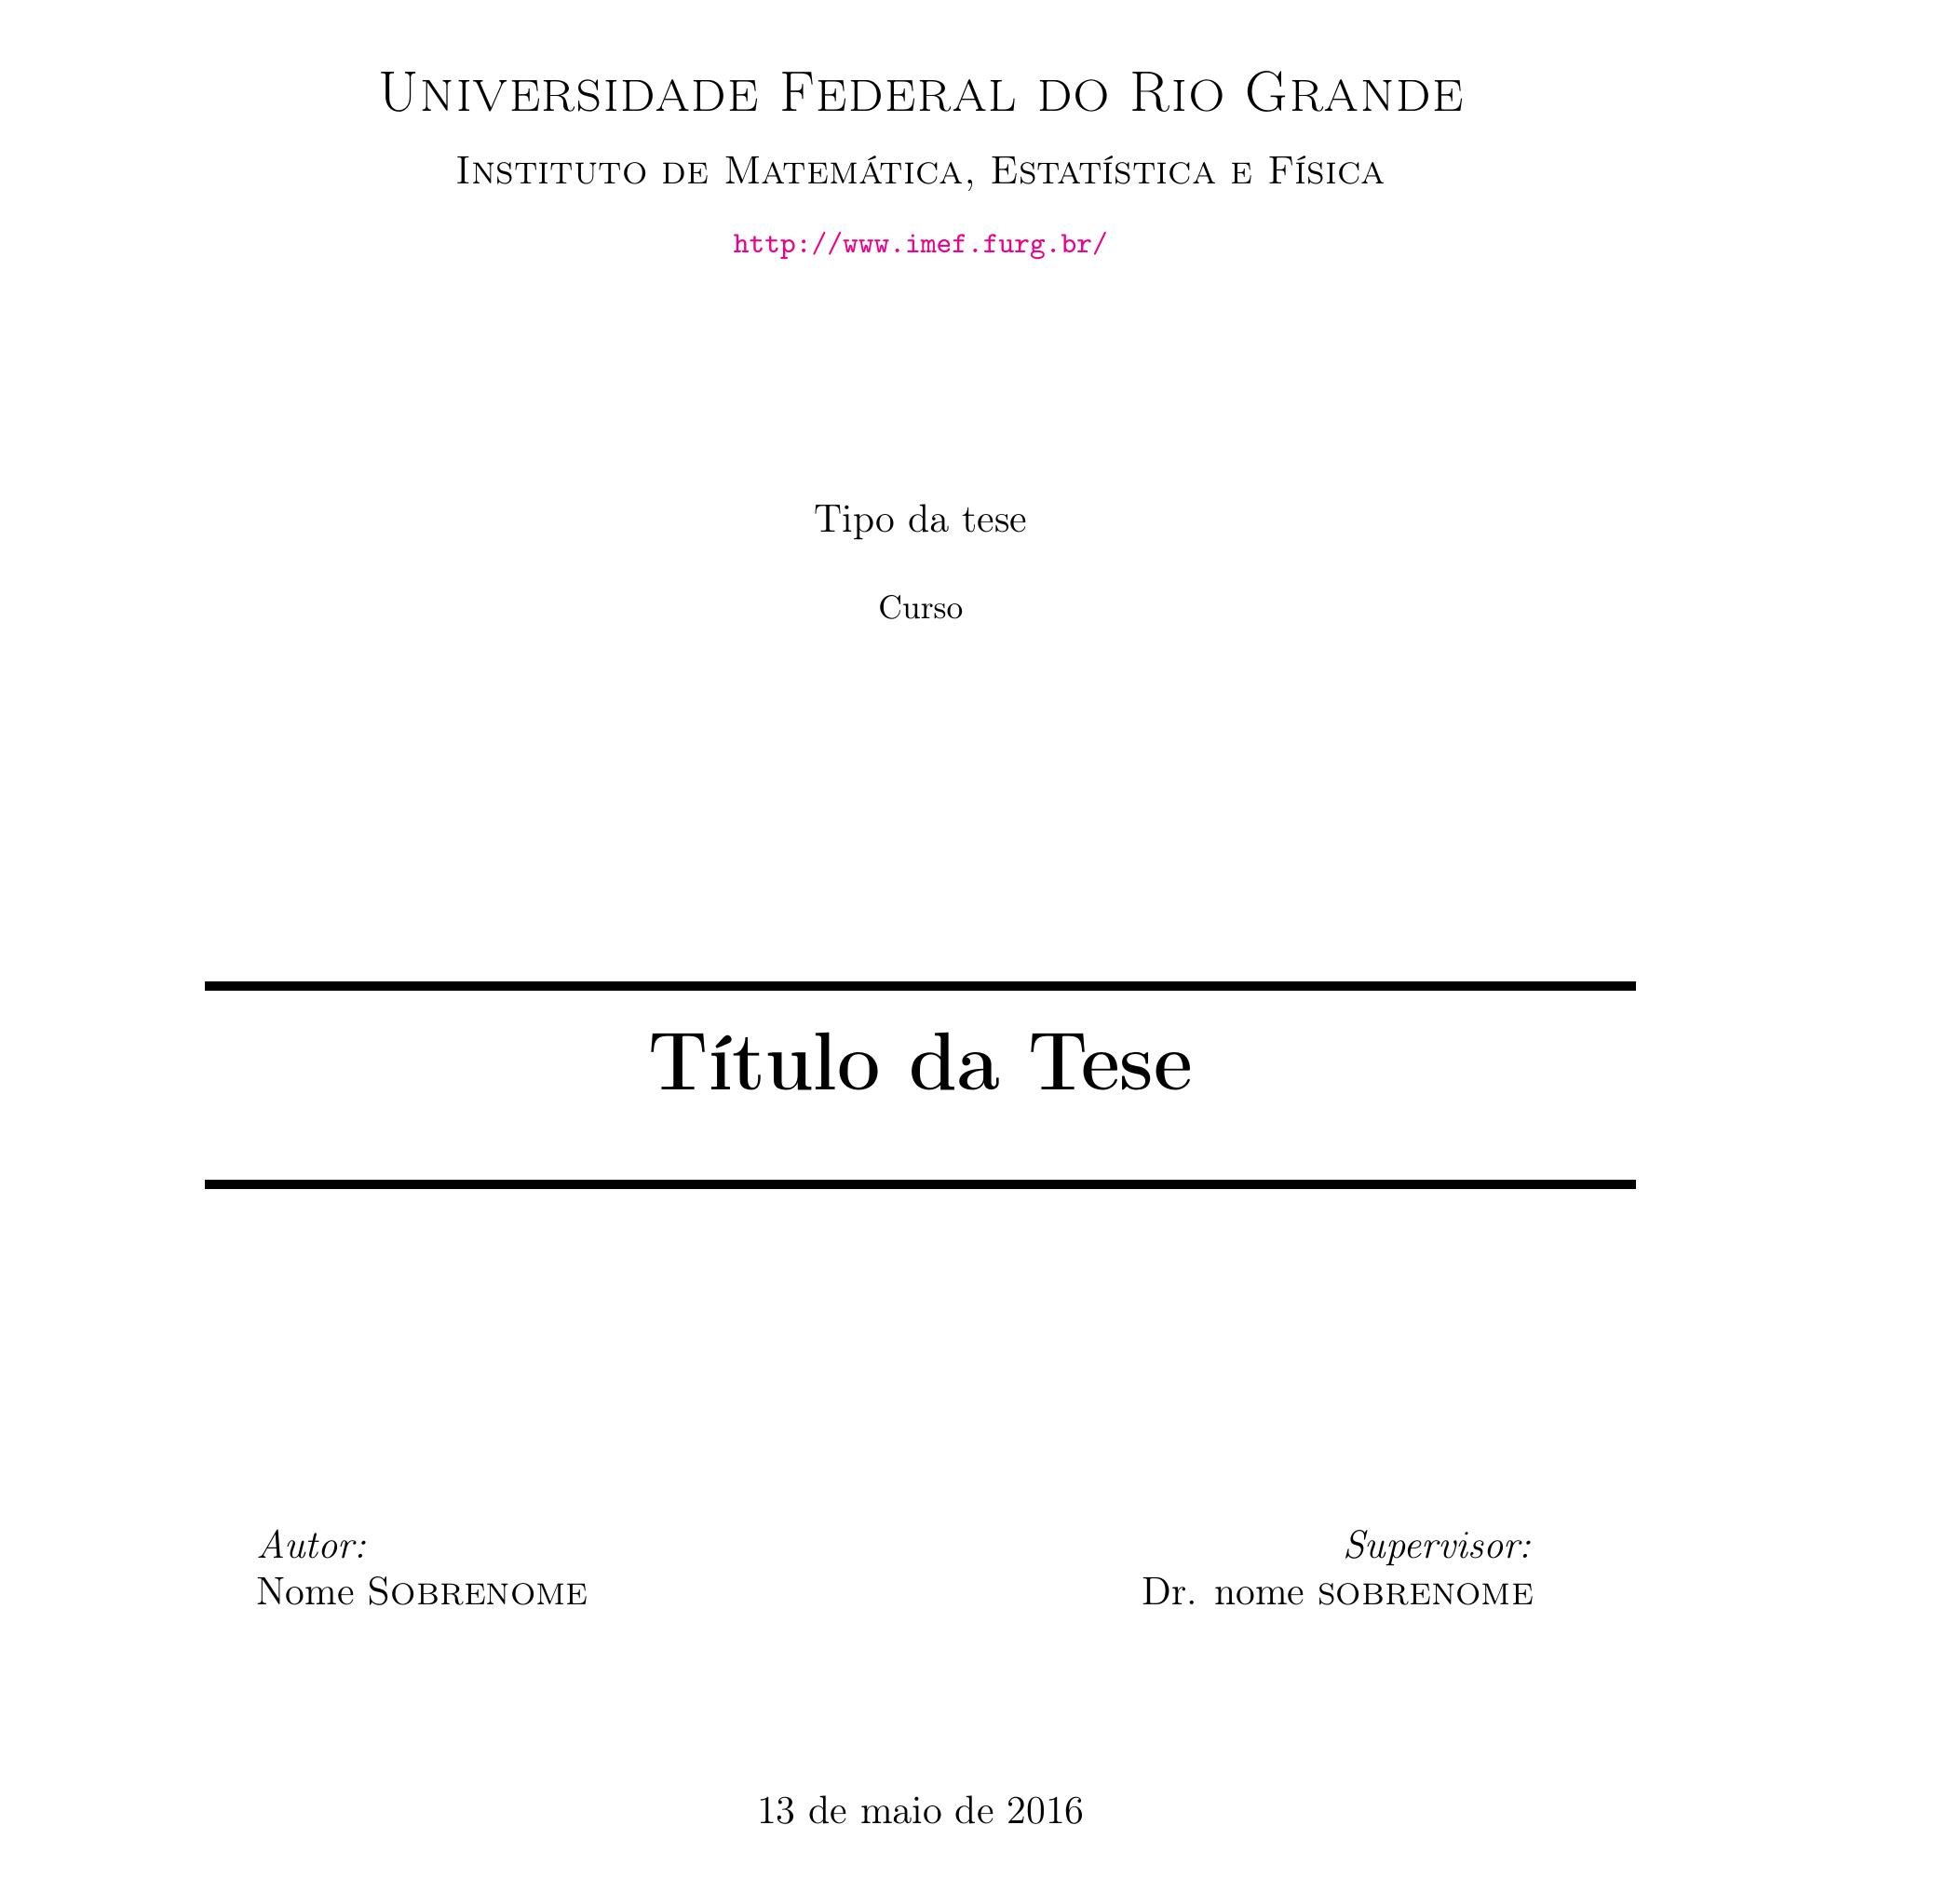
\includegraphics[width=0.60\textwidth]{tese_model.jpg}
% \captionof{figure}{}
\end{center}
\end{frame}






\subsubsection{Artigos e Teses}

\begin{frame}
 
\end{frame}

\subsubsection{Poster}

\begin{frame}
 
\end{frame}

% \section{Referências}
% \begin{frame}{Bibliografia}
% \cite{*}
%  \tiny{\bibliography{l}}
% \end{frame}


\end{document}
\endinput
%%
%% End of file `example_DarkConsole.tex'.
